%% paper.tex


%\documentclass[pldi]{sigplanconf-pldi16}
\documentclass[preprint]{sigplanconf-eurosys}
% standard LaTeX packages

% standard LaTeX packages
%\usepackage{changebar}

\usepackage{balance}
\usepackage{alltt}
\usepackage{amsmath}
\usepackage{balance}
\usepackage{booktabs}
\usepackage{fixltx2e}
\usepackage{graphicx}
\usepackage{boxedminipage}
\usepackage{hyperref}
\usepackage{nicefrac}
\usepackage{subfig}
\usepackage{xcolor}
\usepackage{setspace}
\usepackage{xspace}
\usepackage{multirow}
\usepackage{colortbl}
\usepackage{amsfonts} 
\usepackage{blindtext}
\usepackage{chngpage}
\usepackage{listings}
\usepackage{mathtools}
\usepackage{amssymb}
\usepackage{pifont}

%\captionsetup{compatibility=false}
%\usepackage{pgfplotstable}

\usepackage[linesnumbered, vlined, ruled]{algorithm2e}
% font selection
%\usepackage{courier}
%\usepackage[scaled]{helvet}
\usepackage{mathptmx}
\usepackage{times}

% custom packages for this paper
%\usepackage{double-blind}
\usepackage{shared-affiliation}

\usepackage[numbers,sort&compress,square]{natbib}
%\newcommand{\wenfei}[1]{\textcolor{red}{$<<$Wenfei: #1$>>$}}

\lstset{
  basicstyle=\tiny,
  columns=fullflexible,
  numbersep=5pt,
  numberstyle=\scriptsize,
  showstringspaces=false,
  escapeinside={/*@}{@*/},
  belowcaptionskip=1\baselineskip,
  language=C,
  showstringspaces=true,
  keywordstyle=\bfseries,
  commentstyle=\itshape,
}


%\pgfplotstableset{
%    color cells/.style={
%        col sep=comma,
%        string type,
%        postproc cell content/.code={%
%                \pgfkeysalso{@cell content=\rule{0cm}{2.4ex}\cellcolor{black!##10}\pgfmathtruncatemacro\number{##1}\ifnum\number>5\color{white}\fi##1}%
%                },
%        columns/x/.style={
%            column name={},
%            postproc cell content/.code={}
%        }
%    }
%}


\makeatletter
\def\@copyrightspace{\relax}
\makeatother

\captionsetup{format=default, font=bf}


\newcommand*{\Scale}[2][4]{\scalebox{#1}{$#2$}}%
\newcommand{\comment}[1]{{}}



%% taken from unknown.sty
%\DeclareCaptionType{copyrightbox}

\sloppy

\input macros.tex

\begin{document}



\title{
  Understanding Malwares and Anti-Virus Engines in the Real World
}

%\numberofauthors{2}
\authorinfo{Paper ID: XXX}
           {Total Page: XXX}

\maketitle


%\theoremstyle{definition}
\newtheorem{definition}{Definition}[section]


\begin{abstract}
\input section/abstract.tex
\end{abstract}


\section{Introduction}
\label{sec:intro}

There is and will continue to be a constant competition between anti-virus tools and malwares.
Malwares grow exponentially~\cite{avtest} and place an imperative threat to human society. 
For example, more than 390000 new malwares are registered in AVTest institute every day~\cite{avtest}.
As another example, a new type of threat, ransomware, has caused more than 1 billion dollars this year~\cite{ransomware}. 
In order to keep up and detect these new types of malwares, anti-virus tools are also improving rapidly,
by constantly updating their signature database, by using more advanced techniques like deep learning~\cite{cylance}, or by utilizing more data. 

In order to improve anti-virus tools and defend against emerging threats from malwares, 
it is essential to understand malwares and existing anti-virus tools in the real world. 
Previous works on studying malwares and anti-virus engines do provide valuable 
insights~\cite{ZhouSP2012,GuptaComsnets2009, vendors-study} such as  
how malware writers create new malwares and how malwares escape from the detection of anti-virus engines.
However, these previous works only studied limited malwares
%and fail to understand malwares in a large scale, 
and did not provide insights into the relationship between malwares and anti-virus engines. 

We propose to use the vast amount of existing ``big data'' 
to study real-world malwares and their relationship with anti-virus engines.
To conduct such study, we utilized an open data repository
that contains billions of real-world malwares, {\em \vt}.

\vt{} is a free online malware scanning servive
that applies a set of state-of-the-art anti-virus engines to analyze user-submitted files 
and sends a detection report back to user.
\vt{} provides public access to all its submitted files and analysis results. 
\vt{} is a valuable resource to study and 
understand real-world malwares and anti-virus engines. 

First, there are huge amount of suspicious files submitted to VirusTotal. 
%As shown in Figure~\ref{fig:subnum}, 
For example, within our data collection window, 
there were around 40 million submissions to \vt\ each month. 
These submissions cover a large variety of file types, and 
are conducted by a large variety of \vt\ users from all over the world. 
This amount of diverse data on VirusTotal serves as a good representation of malwares in the real world.  

Second, for almost all submissions, 
VirusTotal applies no less than 50 state-of-the-art anti-virus engines to analyze them. 
VirusTotal keeps detailed detection results and provides an open access to these results. 
Analyzing historical detection results can help capture how anti-virus engines evolve over time. 

Third, VirusTotal provides rich metadata for each submission. 
Besides the detection results of various anti-virus engines, 
VirusTotal also provides file type information, submitter information, and a hash string of the original submitted file.
These types of information is valuable to study 
%which can help categorize malwares, 
%source ID (country), which can help understand popularity of malwares, 
%ssdeep digest string, by using which we can calculate code similarity without accessing binary executable, and so on. 

Unfortunately, there has only been limited attention to \vt\ in the past. 
%Researchers have used \vt\ as a testing platform when \yiying{developing malwares?}
Researchers tried to capture malware writers who leverage \vt{} as the testing platform during malware development~\cite{huangvt2016bigdata, neeles}. 
Anti-virus vendors use \vt\ to detect possible false positives and false negatives in their products. 
But none of them study the rich malware data provided by \vt\ in a large scale. 

We collected 4 months of metadata of all submissions to VirusTotal 
and conducted an extensive study on them.
%Following previous works~\cite{SongAPsys2016} on studying VirusTotal,
%We focus our effort on Windows \textit{Portable Executable} ({\em \pe}) files, 
%which account for more than half of \vt{}’s submissions.
After collecting and pre-processing data from \vt, 
we first perform a set of basic analysis to gain an overall knowledge of the \vt\ data repository,
including how big the files submitted to \vt\ are, who submit to \vt, and how many submissions are labeled as malware.

On top of these basic findings, we developed a set of more advanced studies in three directions. 

First, we study the correlation between submissions’ metadata and their {\em detection rates}, 
the percentage of engines labeling a submission as malware. 
We found high correlation between detection rate 
and three factors: submission file size, the history of submitting a file, and the reputation of the submitters.
These results shed light on what types of submission are more likely to be malware.
With this result, future researchers and anti-virus vendors can have more guided direction 
into what they should have further investigation.
%help security experts invest their limited manual efforts, 
%and help anti-virus vendors identify possible false positives and false negatives in their products.   

Second, we study the question of whether or not different anti-virus vendors can influence each other
and if detection rate is a perfect measurement of the likelihood of a file being a true malware.
Anecdotely, anti-virus vendors frequently leverage VirusTotal to identify false negatives in their products, 
which are malwares detected by others’ products but not detected by their own products. 
To verify this hypothesis, we use the detection history from VirusTotal 
and developed statistical models based on a known technique from from the web mining area to quantify the influence between vendors. 
With this method, we confirmed that there do exist high influence between vendors;
certain vendors are highly influenced by the detection results of other vendors and use this information to change their detection results.
This result alerts \vt\ users and researchers to be more careful about the detection results from vendors 
and use detection rate more precautiously.
%Anti-virus vendors can rely on this technique to identify false negatives in their products. 

Third, we explore the feasibility of building malware classifiers or detectors based only on hash values of files.
We obtained hash strings of submitted files to \vt\ 
and use the similarity of these hash string to build classifiers.
%The similarity between two ssdeep hash strings 
%is a good estimation of similarity between the two original binary files.
%If we can build malware detectors by using ssdeep hash strings, 
%we can avoid manually extract signatures from malware samples.   
We design several machine learning experiments to evaluate our hash-based malware classifiers. 
Surprisingly, our evaluation results show that by just using hash string, 
we can obtain high accuracy for certain classification tasks.
At the same time, other classification tasks are not as accurate.
We further developed a mechanism to predict which classification task is likely to have high accuracy.
With these classification and detection mechanisms and the large amount of data,
it will be possible to just use a compressed representation of files instead of the original files 
to detect malware.
This result implies that future users can have higher privacy and do not need to reveal their files to know whether or not they are malware.
%Our evaluation results show that precision of malware classifiers are 
%bounded by percentage of tailing examples and more training data tends to bring better results.

Our study advances the understanding of malwares and anti-virus engines in the real world 
and provides various valuable insights for future researchers and vendors.
%apply machine learning to malware detection in a large scale. 


\section{Data Collection and Basic Analysis}
\label{sec:meth}

This section discusses how we collect data and metadata from VirusTotal
and how we preprocess them.
We also present the analysis results of their basic properties, 
before delving into more advanced analysis in later sections.


\begin{table}[h!]
\centering
\footnotesize
{
\begin{tabular}{l|l}
\hline
Metadata Field & Explanation \\
\hline                            
%\cline{1-1}
{\bf name}      & submitted file name \\
{\bf link}      & where to download the file \\
{\bf timestamp} & timestamp when the submission was made \\
{\bf source\_country} & the country where the submission was made \\
{\bf source\_id} & user ID who made the submission\\
{\bf size} & file size \\
{\bf type} & file type \\
{\bf tags} & labels with more specific information for each {\bf type}\\
{\bf first\_seen} & when the same file was first submitted \\
{\bf last\_seen} & when the same file was last submitted \\
{\bf hashes} & sha1, sha256, md5, and vhash\\
{\bf ssdeep} & ssdeep digest string \\
{\bf total} & number of engines analyzing the file \\
{\bf positives} & number of engines that flagged the file as malicious \\
{\bf positives\_delta} & changes in {\bf positives} across different submissions\\
{\bf report} & detailed detection report from each AV engine \\
\hline
\end{tabular}
}
\caption{VirusTotal Metadata. 
%\footnotesize{
(Fields for each submission retrieved from VirusTotal through distribution API and their related explanation.
One file could be submitted multiple times by different users.)
%}
}
\label{tab:fields}
\end{table}


\subsection{VirusTotal}
\yiying{we need to first introduce VT. what does it do, what does it provide, etc.}
\vt\ is a free online malware detection tool? etc.
It's used widely etc.
It's been around for ** years etc.
It's the only open access to real malwares?
Are users of VT mostly AV companies, software companies, OS companies, normal user, attackers? Do we have any way to tell or guess this?

{\color{red}
\vt is a free online malware scan service, 
which was founded in 2004 and was acquired by google in 2012. 
\vt is very popular in security community. 
Anti-virus vendors use \vt to verify false positives and false negatives in their products.
Users submit suspicious files to \vt to check for viruses possibly missed by their own anti-virus software or false alarms from their anti-virus software.  
}

\yiying{how do people use VT, how does VT use AV engines and generat its report}
For each \pe\ submission, \vt\ uses a set of anti-virus engines to analyze it.

{\color{red}
For each submission, \vt applies a set of anti-virus engines to analyze it. 
\vt keeps information about whether the submission is labeled as malware by each engine, 
and detailed tags for identified malware from each engine. 
}

\vt\ provides open APIs to access and download both the metadata of all submissions and detection results.
These APIs work like a pipe or a callback registering method.
After a user opens the API and establish ** to \vt, \vt\ will keep returning metadata for latest files submitted to the user.
blabla

{\color{red}
\vt provides open APIs to access and download both the metadata of all submissions and detection results.
One API, named distribution API, works like a pipe.
After a user opens the distribution API and starts to download data from \vt, 
\vt will keep returning metadata for latest submission to the user. 
Roughly 20 GB data can be downloaded from \vt through distribution API.  
}

\vt\ provides rich metadata.
Table~\ref{tab:fields} shows the metadata fields and their meaning.  
The original submitted files from \vt\ can be downloaded using the {\bf link} field in the metadata.

\subsection{Data Collection and Preprocessing}
We collected all metadata for all submissions to \vt\ from May 7th, 2016 to September 6th, 2016,
with a total of 151 million submissions. 
\yiying{We need some explanation here about why only four months of data is collected. maybe something like we found four months' data is already enough to make meaningful conclusions?}

{\color{red}
According to Lastline Labs~\cite{Lastline}, a common lag time for an anti-virus engine to detect a new malware is two weeks,
so we think our four months' data is enough for us to draw  meaningful conclusions. 
Our collected data is larger than or comparable to previous works on studying \vt~\cite{SongAPsys2016,huangvt2016bigdata}.
}

We performed our data collection using \vt{}’s distribution API.
We insert all collected metadata into a table in Cassandra~\cite{cassandra} 
using the combination of sha256, source\_id, and timestamp as the key.

\begin{figure}[t!]
\begin{center}
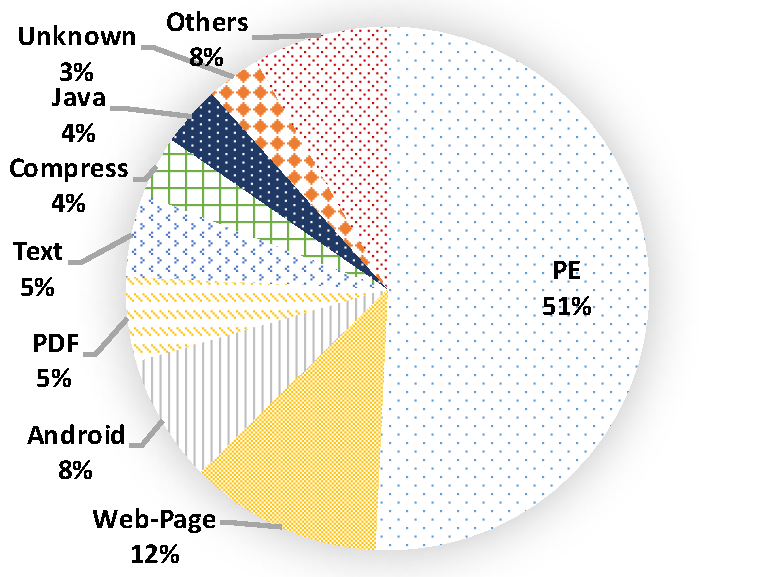
\includegraphics[width=2.in]{figure/type}
\caption{File type distributions.
%{\footnotesize{
(File types and their distributions for all VirusTotal submissions from 05/07/2016 to 09/06/2016.)
%}
}
\label{fig:type}
\end{center}
%\vspace{-0.25in}
\end{figure}


Figure~\ref{fig:type} shows the file type distribution for all submissions. 
Among all file types, Windows \textit{Portable Executable} ({\em \pe}) files, or ``Win32EXE'' and ``Win32DLL'' files, 
are the most frequently submitted type,
accounting for 51\% of all submissions.
%which conforms with a previous study~\cite{SongAPsys2016}.
Web pages and malwares on Android account for the second and third largest submissions, 
with 12\% and 8\% of all submissions respectively. 
Other popular file types include PDF, Text, compressed files, and Java files. 

Since PE files are the most common type,
we focus our study in this paper on \pe\ files 
and leave studies on other types of malwares for future. 
%If the type field for a submission is either ``Win32EXE'' or ``Win32DLL'', 
%we consider the submission is a PE file. 
In total, we collected 76 million \pe\ submissions.

\subsection{Basic Analysis}
After collecting data, we first conducted a set of basic analysis 
to learn the 



\begin{figure}[t!]
\begin{center}
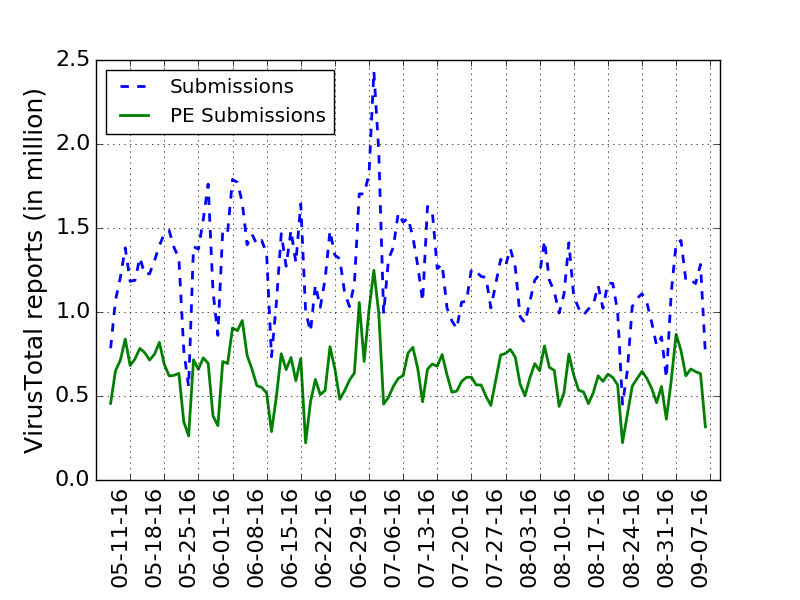
\includegraphics[width=2in]{figure/Submissions}
\caption{The number of files and PE files.
%{\footnotesize{
(The number of suspicious files and the number of PE files submitted to VirusTotal from 05/07/2016 to 09/06/2016.)
%}
}
\label{fig:subnum}
\end{center}
%\vspace{-0.25in}
\end{figure}

\begin{figure}[t!]
\begin{center}
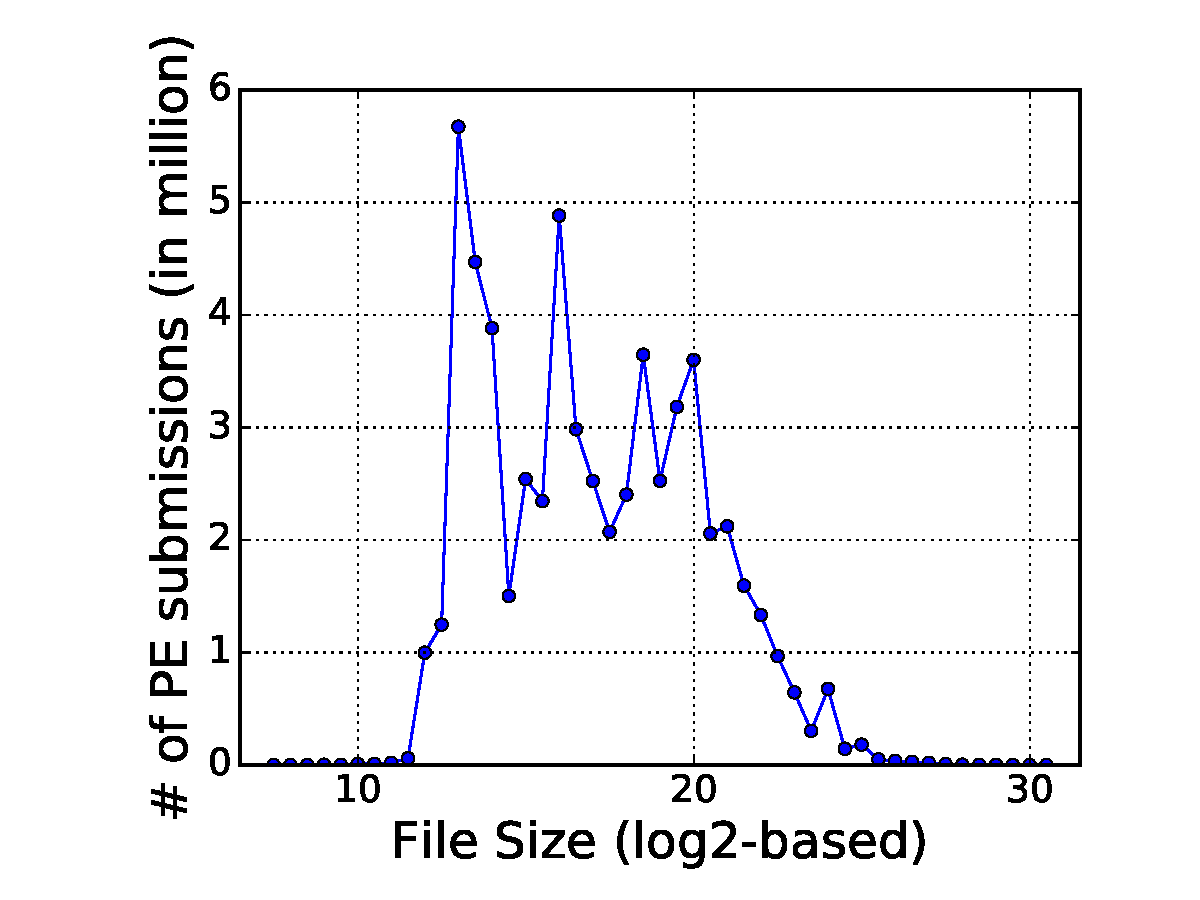
\includegraphics[width=2.5in]{figure/pesize}
\mycaption{fig:pesize}{File size distribution for PE submissions.}
{\footnotesize{(How file size distributes among all PE submissions we collect. 
Results from log2 are rounded up to nearest 0.5.)}}
\end{center}
%\vspace{-0.25in}
\end{figure}
\noindent{\bf Submission temporal, geo-location, and size distribution.} 
Figure~\ref{fig:subnum} plots the number of submissions of all types and the number of \pe\ submissions per day 
over the whole collection period.
There are a large amount of submissions every day
and the amount of submissions is fairly stable over the whole collection period.
The same conclusion can be made to \pe\ submissions.

\yiying{we still need the country distribution}

Figure~\ref{fig:pesize} shows the file size distribution for PE submissions. 
The smallest PE file is only xxx bytes, and the largest one is more than xxx\,MB. 
xxx\% of PE file fall into the range from xx\,KB to xx\,MB. 

\begin{figure}[t!]
\begin{center}
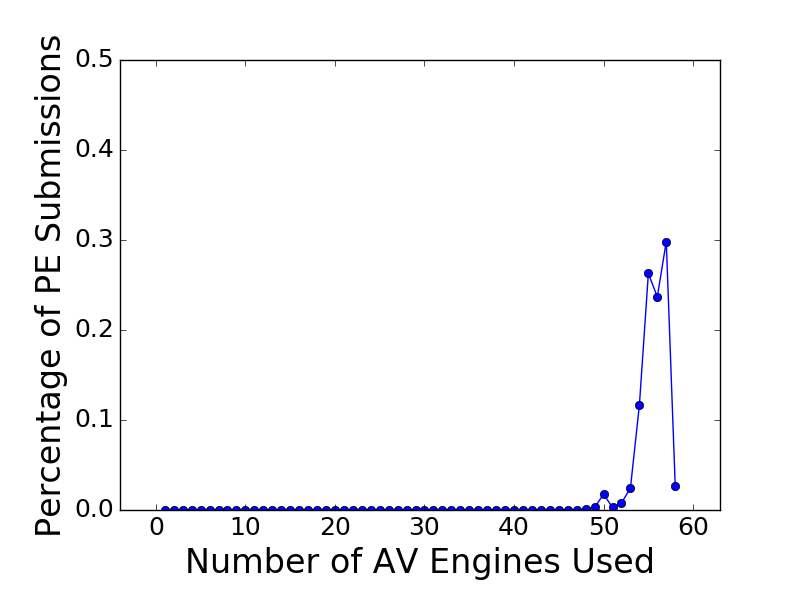
\includegraphics[width=2in]{figure/numVendor}
\caption{The distribution for the number of used anti-virus engines.
(How the number of applied anti-virus engines distributes among all PE submissions.
)
}
\label{fig:vendornum}

\end{center}
%\vspace{-0.25in}
\end{figure}
\begin{figure}[t!]
\begin{center}
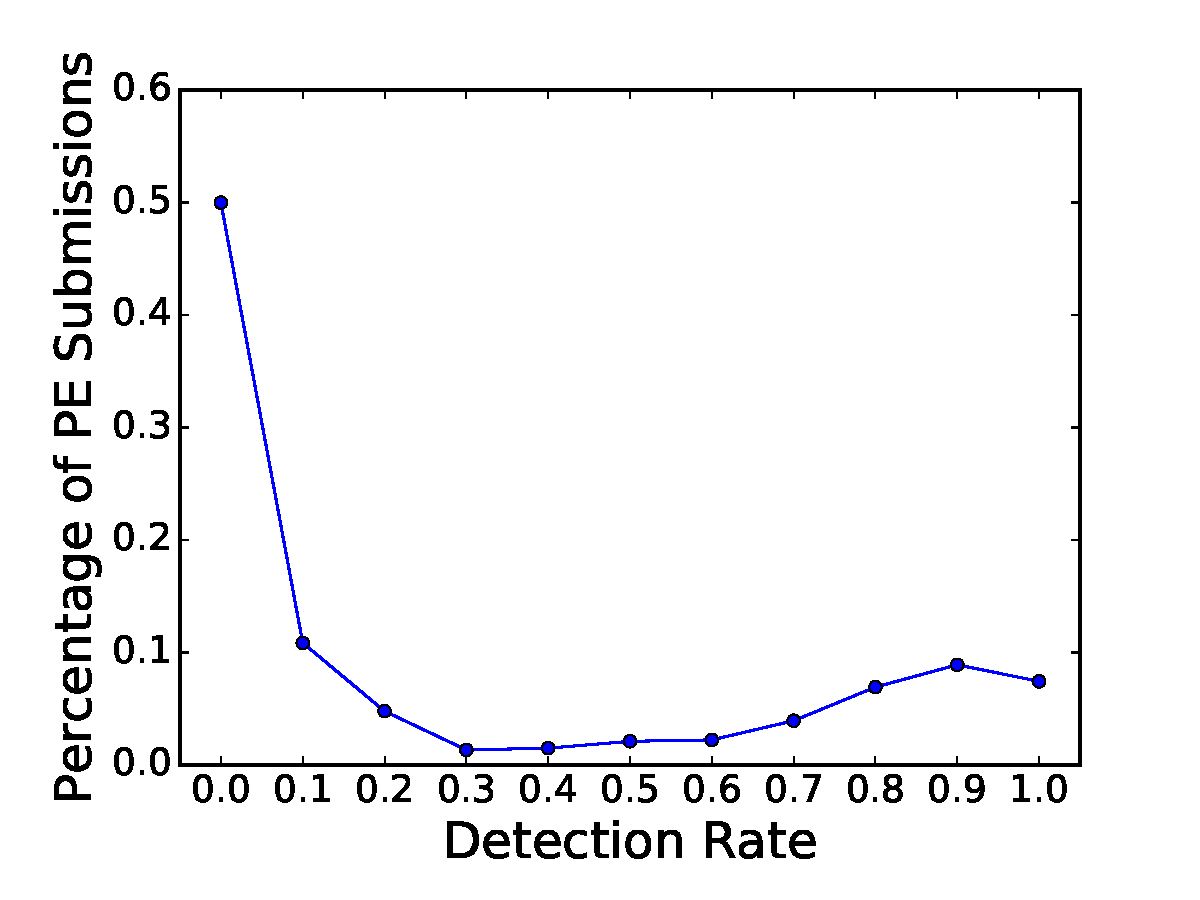
\includegraphics[width=2in]{figure/DetectionRate}
\caption{The distribution for detection rate.
(How detection rate distributes among all PE submissions. 
Each detection rate is rounded up to nearest 0.05.)
}
\label{fig:detectiorate}
\end{center}
%\vspace{-0.25in}
\end{figure}
\noindent{\textit{\underline{Anti-virus engines and detection basic analysis.}}}
%As shown in Table~\ref{tab:fields}, 
%total field is to represent the number of used anti-virus engines. 
Figure~\ref{fig:vendornum} shows the distribution for the number of used anti-virus engines. 
More than 99\% of PE submissions are analyzed by at least 50 anti-virus engines. 
Some anti-virus engines will label a submitted PE file as malware, 
while others will not. 
Positives field in Table~\ref{tab:fields} represents the number of anti-virus engines labeling the submission as malwares. 

$$ \textrm{\textit{Detection Rate}} = \dfrac{positives}{total + 1}$$

Detection rate represents the percentage of engines labeling the submission as malware. 
Adding one to total is to avoid dividing 0 exception, and more importantly, 
to give submissions labeled as malwares by more engines higher detection rate. 
For example, after adding one, submissions analyzed by 50 engines and detected by 50 engines will have a higher detection rate 
than submissions analyzed by 1 engine and detected by 1 engine. 
This formula shares the same intuition from previous work~\cite{GuoICSE2010}, when computing reputations for bug reporters. 
A larger detection rate usually indicates a more malicious malware suggested by analyzed anti-virus engines. 
Figure~\ref{fig:detectiorate} shows how detection rate distributes among all PE submissions. 

One PE file could be submitted more than once to VirusTotal. 
There are 6.72\% PE files submitted more than once to VirusTotal. 
On average, each PE file is submitted 1.19 times. 
Some anti-virus engines may produce different detection results when analyzing the same file for different submissions.
We assume there is influence among different anti-virus vendors, 
and this influence is a very important reason causing engines to change their results.
We will discuss how we model this influence and how to predict possible detection result change by using our model in Section~\ref{sec:influ}.

\subsection{Threats to validity}
\yiying{I don't know what to call this paragraph. But it should go into a subsection}

{\color{red} Another possible section name is Caveats}

Like all other empirical study works, 
our findings and conclusions need to be considered with our methodology in mind. 
We use distribution API to download submissions' metadata from VirusTotal. 
There is no guarantee that all data can be successfully downloaded. 
It could be possible that some files are submitted to VirusTotal, 
but we fail to get their information from VirusTotal.
Although we have collected huge amount of malware information from VirusTotal,
we do believe that there are malwares never submitted to VirusTotal, 
or submitted to VirusTotal much later than they appear in the real world. 
However, there are no conceivable ways to study them.
We believe the 4-month malware information we collect can serve as a representative sample for malwares in the real world. 

\section{Correlation between Submission Properties and Detection Rate}
\label{sec:corr}
This section presents our study of the correlation between various properties of \pe\ submissions and the detection rate of \pe\ submissions.
Detection rate is what most \vt\ users use to decide whether their submissions are benign or malware 
and the first thing that a user of \vt\ uses.
Therefore, it is important to study what factors affects or correlates to detection rate
and the results can guide security researchers and vendors to have targeted investigation over {\em suspicious} files, 
files that have the factors that we identify as highly correlated to detection rate.

We studied a range of properties and their correlation with detection rate
and found that three factors have higher correlation:
submission file size,
historical submission properties, and the reputation of source IDs.
We present these correlation study results in this section.
In the next section, we will present our further analysis of what can affect the detection result of anti-virus engines
and if detection rate is a perfect measurement of the likelihood of malware.

\begin{figure}[t!]
\begin{center}
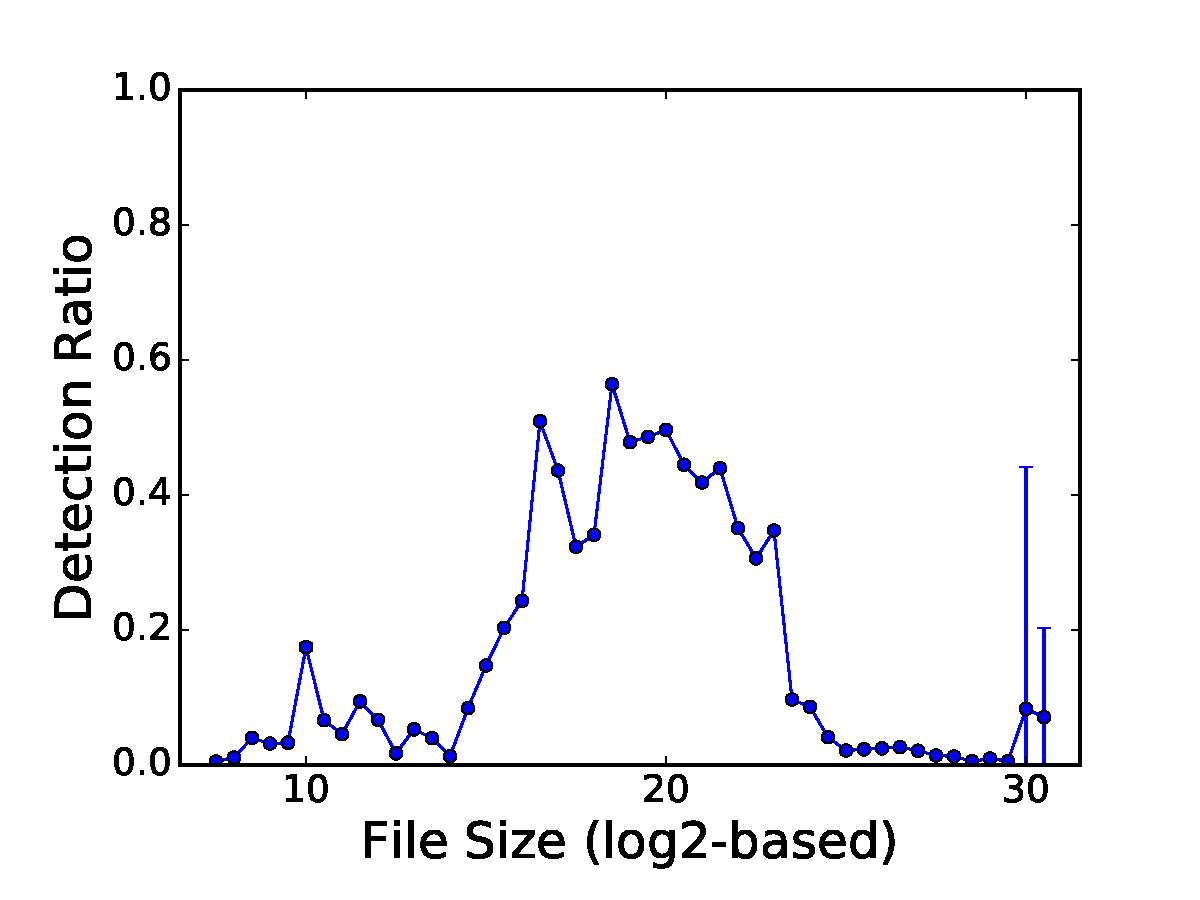
\includegraphics[width=2in]{figure/size}
  \caption{How detection rate changes with file size.
(
95\% confidence interval is also drawn for each point.
Results of log2 for the original file sizes are rounded to the nearest 0.5 value.)
}
\label{fig:size}
\end{center}
%\vspace{-0.25in}
\end{figure}


\subsection{File Size}
\label{sec:size}
Anecdotally, \pe\ malwares are most likely to have small to medium size. 
To verify this, we analyzed the relationship between submission file size and detection rate. 
Figure~\ref{fig:size} presents the average detection rate and 
the 95\% confidence interval for different file sizes.
A wider confidence interval implies that
the calculated average detection rate is farther away from the real average detection rate.
We use discrete file sizes of powers of two in our analysis and in this graph,
i.e., we calculate the log2 of each original file size and round it to the nearest 0.5 value.
Overall, we find that files with size from 90KB to 4MB have higher detection rate, more than 20\% on average. 
Except for the last two points which represent a small amount of files that are bigger than 1GB, 
all other sizes have high confidence.   

{\bf Observation 4:} 
{\em \pe\ malwares are mostly likely to have small to medium size.}

An immediate question to raise is whether the high detection rate of files with small to medium size
is because these files also contribute to most of the submissions as shown in Figure~\ref{fig:pesize}.
As we will discuss in Section~\ref{sec:history}, the correlation of submissions and detection rate is more complex and non-linear.
Thus, there is a more fundamental reason behind the file size correlation with detection rate.
One likely reason of this correlation is that files that are too small are not enough to express the
malware functions while files that are too big are difficult to spread.

\subsection{Submission History}
\label{sec:history}

%\begin{figure*}[!htb]
\minipage{0.31\textwidth}
  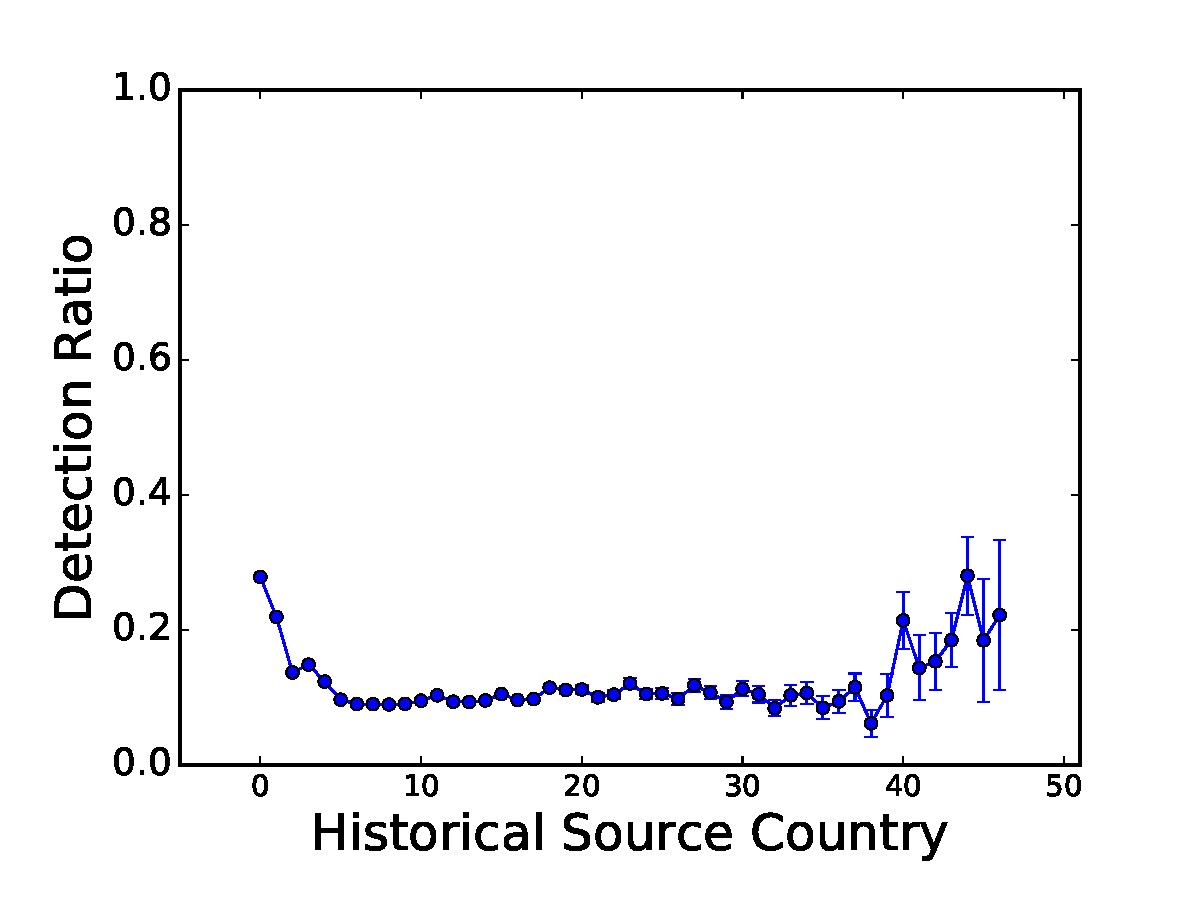
\includegraphics[width=\linewidth]{figure/SubCountry}
  \mycaption{fig:hiscountry}{The relation between the number of historical source countries and detection rate.}
{\footnotesize{(How detection rate changes with the number of historical source countries.
95\% confidence interval is also drawn for each point.)}}
\endminipage\hfill
\minipage{0.31\textwidth}
  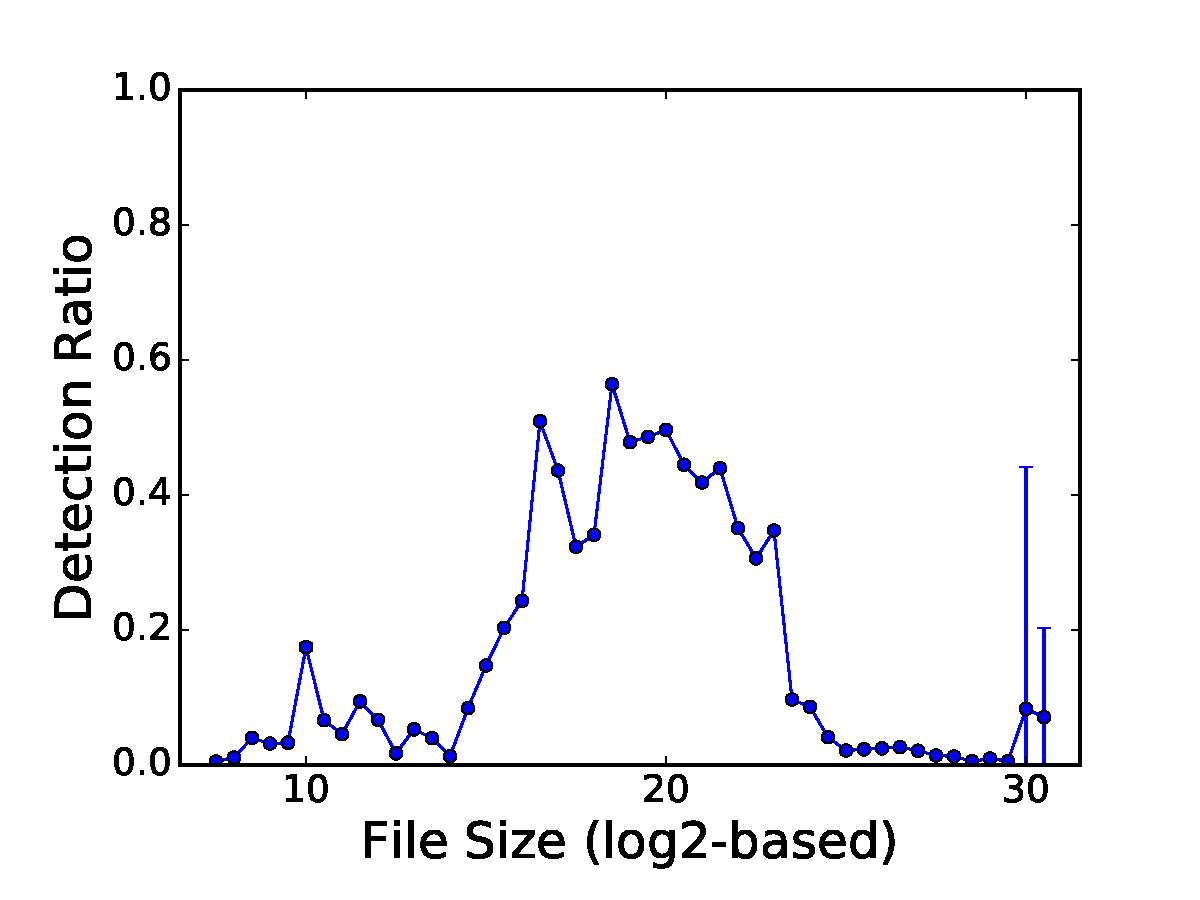
\includegraphics[width=\linewidth]{figure/size}
  \mycaption{fig:size}{How detection rate changes with file size.}
  {\footnotesize{(How detection rate changes with log2-based file size.
Results from log2 are rounded up to nearest 0.5.
95\% confidence interval is also drawn for each point.)}}
\endminipage\hfill
\minipage{0.31\textwidth}%
  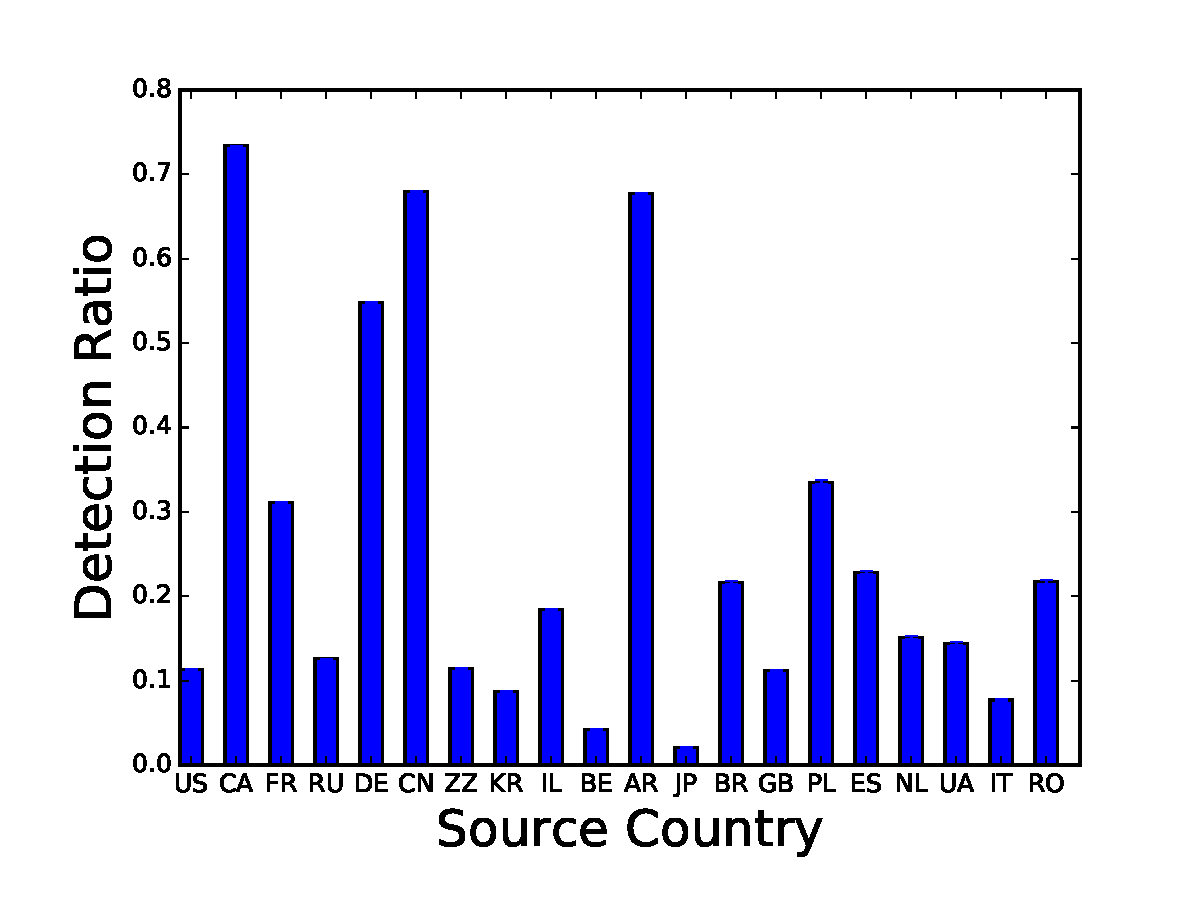
\includegraphics[width=\linewidth]{figure/Country}
  \mycaption{fig:Country}{Average detection rate for top 20 countries.}
{\footnotesize{(Average detection rate for submissions from countries ranking 
in top 20 in making PE submissions to VirusTotal. 
95\% confidence interval is also drawn for each country.)}}
  %\label{fig:aveUncover}
\endminipage\hfill

%\vspace{-0.2in}
\end{figure*}



\begin{figure}[t!]
\begin{center}
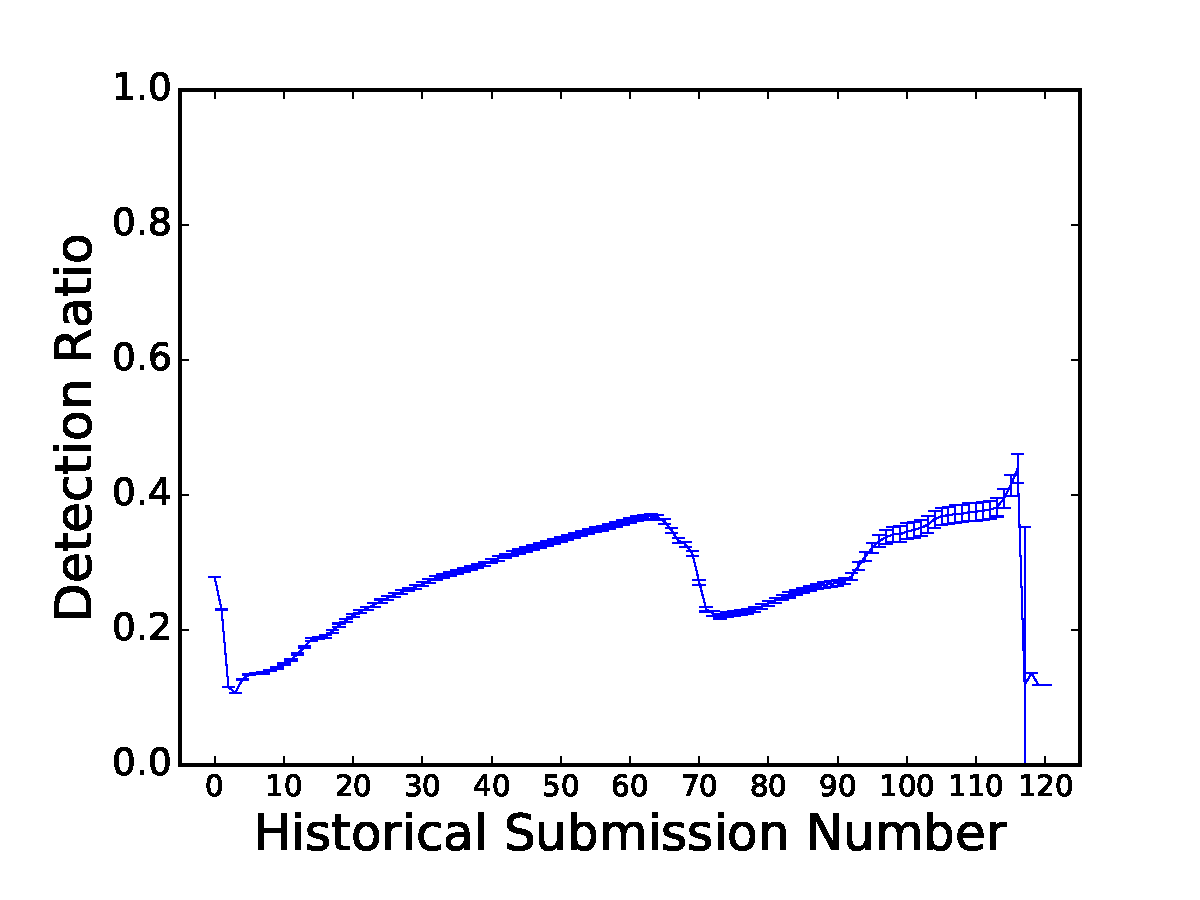
\includegraphics[width=2in]{figure/SubNum}
\caption{
The relation between historical submission number and detection rate.
(
How detection rate changes with historical submission number. 
Each historical submission number is rounded up to nearest 5.
95\% confidence interval is also drawn for each point.
)	
}
\label{fig:hisnum}
\end{center}
%\vspace{-0.25in}
\end{figure}

%\begin{figure}[t!]
%\begin{center}
%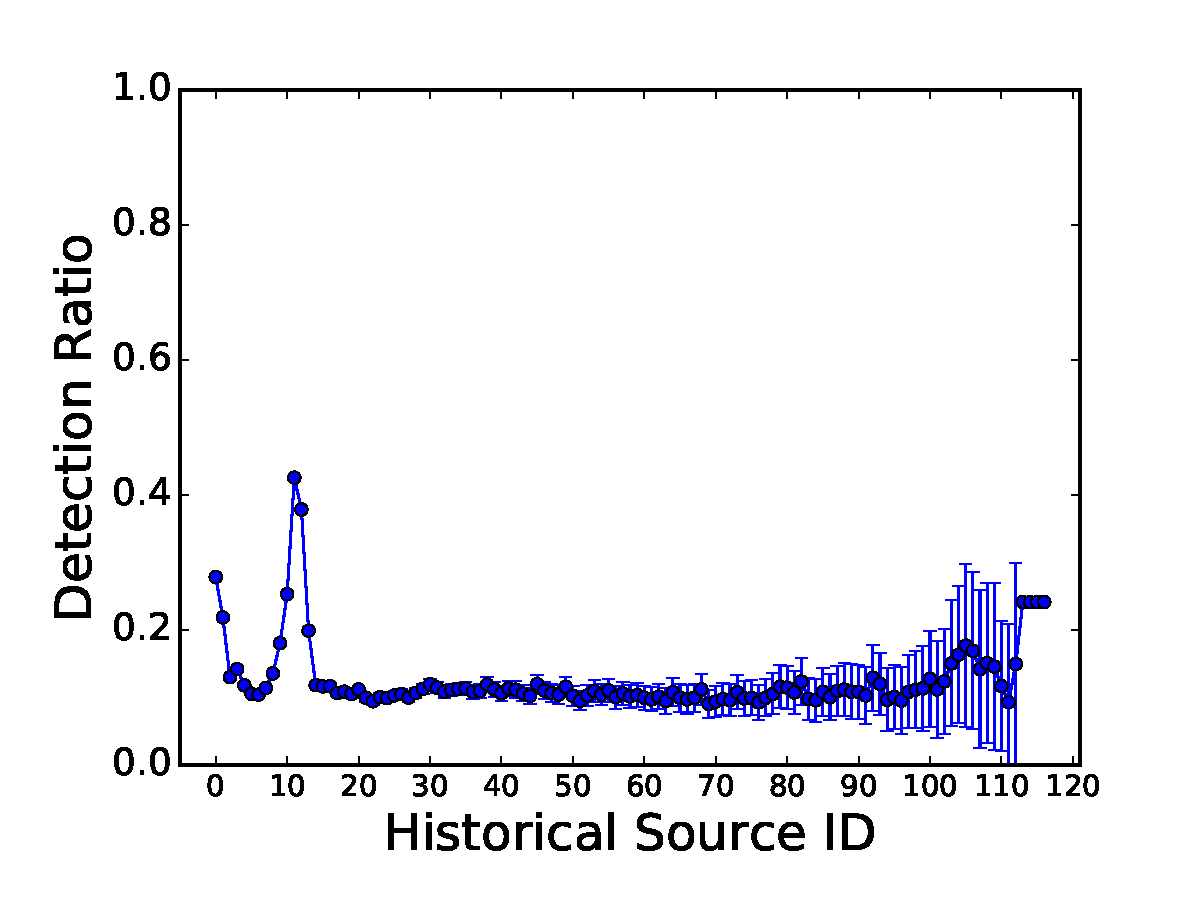
\includegraphics[width=2.5in]{figure/SubID}
%  \mycaption{fig:hisid}{The relation between the number of historical source ids and detection rate.}
%{\footnotesize{(How detection rate changes with the number of historical source ids. 
%Each historical number of source ids is rounded up to nearest 5.
%95\% confidence interval is also drawn for each point.)}}

%\end{center}
%\vspace{-0.25in}
%\end{figure}


As discussed in Section~\ref{sec:basicanal}, there are files that have been submitted more than once to VirusTotal. 
It is worthwhile to investigate this {\em history of submission} and how history affects future.
We study the correlation between submission history and the detection rate of the current submission.
Among the different types of historical information that we study,
we find that two types have higher correlation to detection rate:
the number of submissions made in history and the number of source IDs that made submissions of the same file in history.
%Given a submission, we also study whether information for historical 
%submissions of the same file influences detection rate for the current submission. 

\noindent{\textit{\underline{The number of submissions in history.}}}
To study the submission history, we first sort all submissions for each file chronologically
and then collect the number of all submissions made before submission $s$ for each submission $s$ in \vt.
Next, we calculate the correlation between detection rate and the number of submission in history.
Figure~\ref{fig:hisnum} plots how detection rates change over the number of historical submissions.
Interestingly, there are two main ranges that steadily increase and there are three drops in the beginning, middle, and end.

To explain this effect, we first look at the two factors that can both influence detection rates:
the percentage of benign files submitted and the amount of anti-virus engines labeling the submission as malware.
%Two factors can influence detection rates and explain the above effect.
Obviously, with more benign files submitted, detection rate will decrease.   
and with more engines labeling malwares, detection rate will increase. 
In the the two stages of detection rate increasing, 
with more submissions, more engines are able to identify malwares 
and the increase of percentage of engines identifying submitted malwares dominates. 
In the range that detection rate drops, 
VirusTotal users stop submitting files that have already been identified as malwares,
and the increase of percentage of benign files submitted to VirusTotal dominates. 

%\noindent{\textit{\underline{Number of submitted source IDs in history.}}}
%One file can be submitted by one source ID multiple times 
%and can also be submitted by different source IDs multiple times. 
%We now study the correlation between the number of source IDs in the submission history and the detection rate. 

%\yiying{the whole explanation for this figure needs to be filled here.}
%Figure~\ref{fig:hisid} plots the detection rate and confidence interval as the number of historical source IDs increases. 
%Confidence intervals increases when there are more than 50 source IDs. 
%Detection rate is higher for historical source IDs less than 12, compared with historical source IDs more than 12.
%{\color{red} The X for the largest point is 11. }
%\yiying{is it 12? I cannot tell for sure by just looking at the figure}
%The number of historical source IDs reflects the popularity of a submitted file.
%When the popularity of a file is larger than a certain value, 12 for our dataset, 
%file popularity is unrelated to detection rate. 
%{\color{red} When a file is submitted more than certain number of users, or popular than centain threshold, 
%it is likely to be thoroughly analyzed by all engines, and all vendors have made their decision. 
%They either consider the file as malware or not. They will not change decision. }
%\yiying{why?}

{\bf Observation 5:} 
{\em {\color{red} When historical numbers fall into certain range, they are correlated with detection rate. }}

\if 0
\noindent{\textit{\underline{Historical source country.}}}
One file could also be submitted from different countries. 
The number of historical source countries also reflect the popularity of a submitted file. 
The correlation between detection rate and the number of historical source countries in 
Figure~\ref{fig:hiscountry} shows similar trend as the correlation between detection rate 
and the number of historical source IDs in Figure~\ref{fig:hiscountry}. 

Figure~\ref{fig:hisnum}, Figure~\ref{fig:hisid}, and Figure~\ref{fig:hiscountry} show that 
when historical numbers fall into certain range, they are correlated with detection rate. 
\fi

\subsection{Reputation of Source ID}
\label{sec:reputation}



\begin{figure}[t!]
\begin{center}
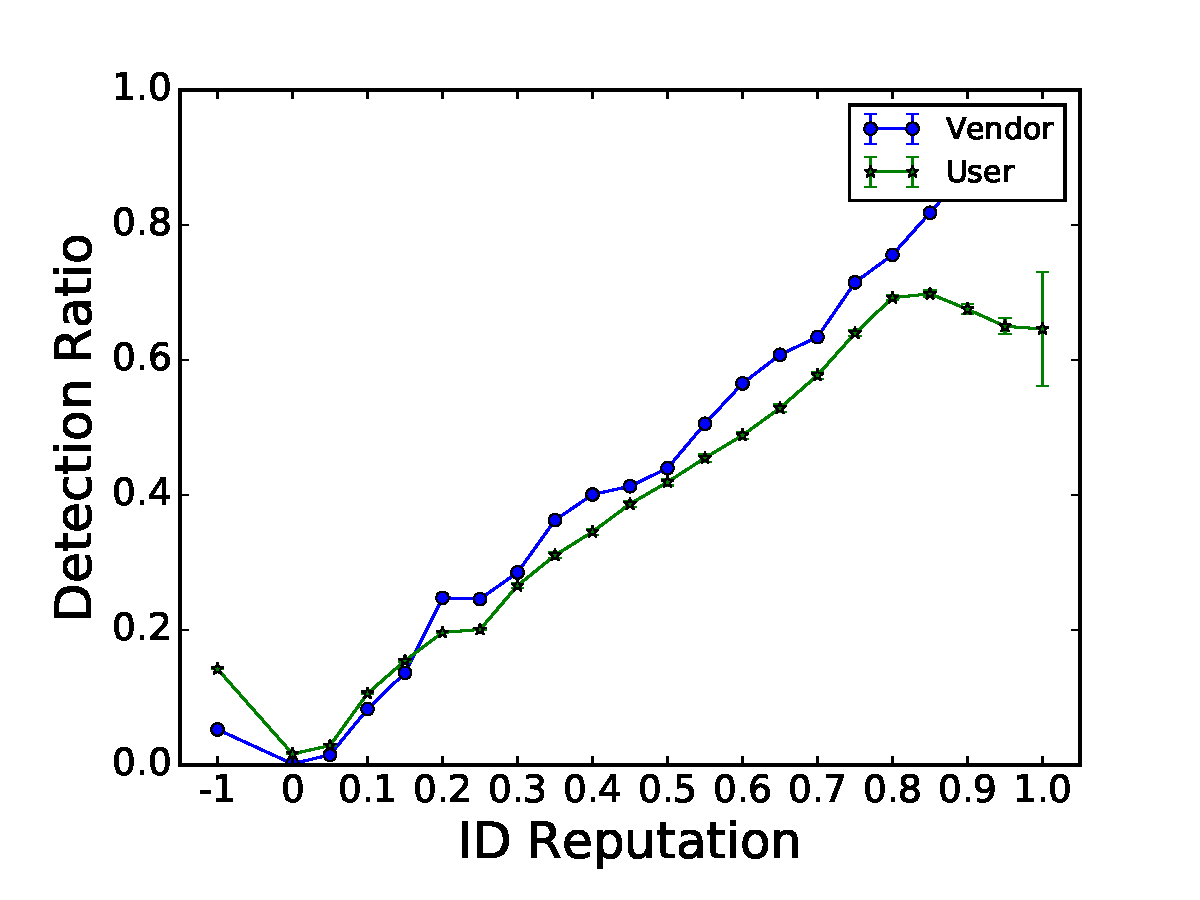
\includegraphics[width=2in]{figure/IDReputation}
\caption{The relation between source id's previous reputation and detection rate.
(How detection rate changes with the value of source id's reputation. 
Each reputation is rounded up to nearest 0.05.
Reputation -1 means the source id did not make any submission before. 
95\% confidence interval is also drawn 
for each point.)
}
\label{fig:idreputation}
\end{center}
%\vspace{-0.25in}
\end{figure}

Different users of online services such as \vt\ often have different {\em reputation} 
because of different motivations, objectives, and backgrounds.
For example, some users can randomly trying out \vt\ with no specific objective and thus submit random files
while other users have clear goals and motivations and thus only submit suspicious files.
The rationale behind reputation is that \vt{} users would have a roughly constant submission pattern, 
and it is promising to use their historical submission to predict their future submission.
Previous work~\cite{GuoICSE2010} reported that there is a correlation between bug reporter’s reputation and the likelihood for the bug being fixed. 
We also observe correlation between the reputation of source ID and submission’s detection rate. 

Intuitively, a user that have submitted more files that were detected as malware suggest 
that she is more likely to use \vt\ to detect malwares in suspicious files 
and thus should be given higher reputation.
To quantify this, we define the reputation of a source ID as the follow.
The reputation of a source ID is not a fixed value and can change over time. 

%\theoremstyle{definition}
\begin{definition}{Reputation:}
Given a submission $S$ with source ID $N$, 
we define the reputation of $N$ when conducting the submission $S$ as the average detection rate for all submissions conducted by $N$ before $S$. 
If $N$ did not make any submission before, we define the reputation to be $-1$. 
\end{definition}

Before conducting our source ID reputation analysis, we first filter out submissions without source ID information (for a small amount of submissions, \vt\ fails to provide source ID),
files that are only submitted once, and files that are submitted more than 1 million times (bogus or robots).
%For around 14\% PE submissions, VirusTotal fails to provide source ID information. 
%We filter out these submissions, when computing reputation.
%All other PE submissions are conducted by 613 thousand source IDs. 
%66\% source IDs only conduct submission once. 
%We filter source IDs conducting more than 1 million PE submissions in our data set, 
%because we think these are anti-virus vendors routinely test their products. 
To calculate source ID reputation, we first sort all submissions from the same source ID chronologically, 
and calculate reputation for each source id when conducting each submission. 
We further separate normal users from vendors and analyze the correlation of their ID reputation and detection rate.

Figure~\ref{fig:idreputation} plots the average detection rate and the 95\% confidence interval 
as the source ID reputation increases for normal users and for anti-virus vendors.
We round up reputation values to their nearest 0.05 values. 

Detection rate steadily increase as the reputation increases from 0 to 1 for vendors and from 0 to 0.8 for normal users.
Except the points when reputation is 1, all other results have high confidence.
Interestingly, for both normal user and vendors the detection rate with reputation -1 is higher than with reputation 0,
which means that the first submissions conducted by all source IDs (reputation -1) 
are overall have higher detection rate than 
the submissions conducted by IDs that have only submitted benign files (reputation 0).

For normal users, the detection rate drops when reputation is greater than 0.8.
This means that for normal users, it is difficult for them to always submit suspicious files detected by almost all vendors.
Vendors do not have this behavior and their detection rate always increases with higher reputation (other than reputation -1).


{\bf Observation 6:} 
{\em There is a high correlation between user reputation and detection rate of their submissions for both normal users and anti-virus vendors.}


\subsection{Discussion}

\noindent{\textit{\underline{How to use our data?}}}
From our analysis, file size, number of submissions in history, and source ID reputation
are all highly correlated with detection rate. 
These results suggest that future researchers and vendors can use these values to have an initial estimation or prediction of future submissions.
Doing so can help reduce researchers' and vendors' effort to focus on more interesting files---files that are more likely to be malicious.
Anti-virus vendors can also inspect results which are variant from our studying results 
to identify possible false positives or false negatives in their products. 

%Linhai, it's not good to say things that you haven't done, esp. in a system paper. so I deleted the regression model discussion
%A possible future work is to train a regression model to combine all these factors together and 
%predict how many engines could detect a malware or how likely a file is a malware. 
%Using the regression model or our studying results alone, 
%security experts can prioritize malwares and focus their efforts on malwares which are more malicious. 
%Anti-virus vendors could inspect results which are variant from our studying results 
%to identify possible false positives or false negatives in their products. 

\yiying{I would delete the following paragraph. it just sounds too defensive. and you've already explained the limitation in sec 2.4.}
\noindent{\textit{\underline{Limitations of our study.}}}
As discussed in Section~\ref{sec:meth}, our study is bound with our methodology.
We do not have any data before 05/07/2016, 
which may cause some inaccuracy in measuring historical statistics and 
source ID reputation and historical numbers.
However, we think we can tolerate this error, 
since we conduct our study in a relatively long time range and in a large scale. 
%In the future, we could design our reputation and historical metrics based on a tunable time windows, and investigate whether correlations still exist.   

\section{Influence Propagation}
\label{sec:influ}

As we discussed in Section~\ref{sec:meth}, 
many files are submitted to VirusTotal more than once, 
and more than 99\% submissions are analyzed by at least 50 anti-virus engines. 
We observe that some engines fail to identify some malwares during early submissions, 
but they catch up when analyzing later submissions. 
Anti-virus vendors frequently use VirusTotal to identify false negatives in their products, 
which are malwares they fail to detect but detected by other vendors. 
We assume that there are influence among different anti-virus vendors.
In this section, we try to model this influence,
and try to predict whether an engine will identify a file as malware in the future, 
after the engine has already labeled the file as benign.

\subsection{Influence Model}
\label{sec:model}

Influence propagation on social graph is a well-studied topic in web mining area. 
The static models we apply are proposed by~\citet{Influence} to analyze Flickr data.
In this section, we will first overview the static models~\cite{Influence} in our usage scenario, 
and then we will discuss how we use map-reduce to train models and use trained models to do prediction.  

We assume that all vendors form a complete directed social graph $G = (V, E)$, 
where the nodes $V$ are vendors. 
The social graph is complete, 
since we assume there is possible influence from any vendor to all other vendors.
We assume there are action logs generated, 
when VirusTotal applies a set of anti-virus engines to analyze a submission. 
For each engine, there will be an action log $(u, a, t)$ or an action log $(u, \bar{a}, t)$, 
representing whether or not $u$ takes action to identify the submission as a malware at time $t$. 
To make things easy, after a vendor $u$ labels a file as malware, 
we assume $u$ will insist its decision, 
and ignore cases where a vendor labels a file as malware, but labels the file as benign later. 

We use $A_u$ to represent the number of actions taking by u, 
or the number of malwares identified by $u$. 
We use $\bar{A}_u$ to represent the number of malwares ever analyzed and labeled as benign by $u$.
We use $A_{u\&v}$ to represent the number of actions taken by both $u$ and $v$, 
and $A_{u|v}$ to represent the number of actions taken by either $u$ or $v$.
Clearly, $A_{u|v} =   A_u + A_v - A_{u\&v}$
We use $A_{u2v}$ to represent the number of actions propagated from $u$ to $v$. 
We define action propagation as follows: 

\begin{definition}{Action Propagation:}
We say that an action $a$ propagated from $u$ to $v$ iff: (i) $\exists$ $(v, \bar{a}, t_i)$ $\in$ $\bar{A}_v$, 
and $(v, a, t_k)$ $\in$ $A_v$, with $t_i < t_k$; (ii) $\exists$ $(u, a, t_j)$ $\in$ $A_u$, with $t_j < t_k$. 
\end{definition}

For each edge $(u, v) \in E$ in the social graph $G$, 
there is an influence probability: $p_{u,v}$,
which represent after $u$ takes an action the probability that $v$ will follow $u$ to take the same action. 
Since social graph $G$ is a complete graph, 
all other nodes are all $v$'s neighbors. 
Let us use $S$ to represent the set of $v$'s neighbors, which take an action. 
The probability that $v$ will follow its neighbors to take the same action is

$$p_v(S) = 1 - \prod\limits_{u \in S}(1 - p_{u,v})$$

During training stage, we try to learn $p_{u,v}$ for each edge. 
During prediction stage, we provide a tunable threshold $\theta$. 
For node $v$ without taking an action, 
if $P_v(S)>\theta$, 
we predict $v$ will follow its neighbors to take the action in the future. 



\subsection{Experimental Results}
\section{Malware Classification}
\label{sec:ssdeep}

Machine learning systems are just as good
as the data they consumed---One potential 
use case of the massive amount of data 
available on VirusTotal is to build 
machine learning models for applications
such as malware classifications and
clustering. In this section, we study
the question that {\em Is the data
provided by VirusTotal enough to support
classifications and clusterings tasks?}

Our study reveals both positive and
negative answers to this question---For
some classification tasks, we are able
to build an automatic classifier whose
accuracy is higher than 80\% by just
using the static signature provided by VirusTotal
and we expect the quality to keep increasing
given more data; on the other hand,
we identify some classification tasks
whose accuracy hardly beat random guesses.
We also identify a simple metrics
to predict whether a given task belongs
the high-quality category or the low-quality
category. We hope our study shed lights
on future design of signatures for malware
detection.

%Malware detectors mainly rely on signatures manually extracted by security researchers. 
%ssdeep only takes static binary executable as inputs. 
%If we can build malware detector based on ssdeep similarity, 
%We can reduce or even eliminate manual efforts in malware detection. 


\subsection{Data Collection}

\begin{table*}
  \centering
  \scriptsize
  {
  \begin{tabular}{clccc}
    \toprule
{\bf Index} & {\bf Microsoft Tag} & {\bf \# of Malwares} & {\bf \% of Tailing}  & {\bf \% of Distinct}\\
\midrule                                                                                                                                                                                                                                           
1  &  SoftwareBundler:Win32/Penzievs 	& 49380	     & 3.51\%  & 99.98\%\\
2  &  Adware:Win32/Hotbar               & 132161   & 1.88\%  & 99.98\%\\
3  &  TrojanDropper:Win32/Lamechi!rfn	& 39205	     & 0.01\%  & 6.13\%\\
4  &  Virus:Win32/Nabucur.D	            & 1190132  & 99.95\% & 100.00\%\\
5  &  Virus:Win32/Virut.BO	            & 84600	   & 21.84\% & 99.95\% \\
6  &  Worm:Win32/Mydoom.L@mm	        & 76259	     & 0\%     & 99.44\%\\
7  &  Virus:Win32/Ramnit.I              & 412052   & 3.07\%  & 96.76\%\\
8  &  Trojan:Win32/Dorv.A               & 54324    & 2.80\%  & 80.53\%\\
9  &  Trojan:Win32/Dynamer!ac           & 145402   & 65.17\% & 99.20\%\\
10 &  Virus:Win32/Ramnit.A              & 181524   & 26.79\% & 99.82\%\\   

\bottomrule
   \end{tabular}
   }
   \mycaption{tab:benchmark}{Benchmark Information.}
{\footnotesize{(Information for malwares used in our clustering and classification experiments. \# of Malwares: \# of distinct malwares we collected in each sampled malware group from 05/07/2016 to 09/06/2016. \% of Tailing: \% of tailing examples in each group. \% of Distinct: number of distinct ssdeep hash strings divided by group size.)}}
  %\nocaptionrule
  %\mycaption{tab:benchmark}{Malware Data Set.}
  %\footnotesize{(Information for malwares used in our clustering and classification experiments. \# of Malwares: \# of distinct malwares we collected in each sampled malware group from 05/07/2016 to 09/06/2016. \% of Tailing: \% of tailing examples for each group in the sampled 10000 malwares.)}
 %}
\end{table*}




Our study uses features based on ssdeep~\cite{ssdeep}, a program to compute fuzzy hashes. 
Similarity between calculated hash strings can serve as an estimation for similarity between the two original files. 
ssdeep hash strings are also provided for each submitted file with other metadata fields by \vt. 

We focus on classifying each malware into
different malware families. Because Microsoft 
has a good reputation in detecting PE malwares~\cite{SongAPsys2016}, we create training
data using its assignment. For each detected malware, Microsoft assigns it a tag, which contains type, platform, family, and variant information~\cite{microsoft}. 
We divide PE malwares detected by Microsoft engine into different groups, and malwares in the same group share the same Microsoft malware tag. 
We sample 10 groups, each of which with more than 10000 malwares.  
Microsoft tag and number of malwares in each sampled group we collected from \vt{} are shown in Table~\ref{tab:benchmark}. 
For each group, we sample 10000 malwares, and use these malwares in our following experiments. 


\subsection{Classification Accuracy}

We build an classifier as follows. \ce{XXXX LINHAI, ADD IN THE PROTOCOL.}

Table~\ref{tab:results} shows the classification
result and Figure~\ref{fig:moredata} shows
the relationship between the amount of
training data and the accuracy of classifiers. 
We see that for five out of ten 
malware families, we achieve an accuracy
higher than 80\%. Moreover, as indicated
by Figure~\ref{fig:moredata}, when more
training data are available for these
families, we expect the accuracy to be even
higher. On the other hand, for
families such as ``Virus:Win32/Nabucur.D'',
the classification accuracy are significant
lower. We get an accuracy of 59\% when
\ce{the accuracy of random guesses would be 50\%. LINHAI IS THIS RIGHT?}
\ce{LINHAI, ADD ONE SENTENCE ABOUT THE REASON.}

\paragraph*{Discussion: Tailing Malwares}

We identify one metrics to predict whether
a classification task falls into the
high-accuracy category or low-accuracy
category. The intuition is that the probability
that a given sample has similar samples in
the training set is a proxy of the upper bound
of accuracy that we can expect. Therefore,
we compute the percentage of tailing malwares in each group--We call malwares, which have 0 similarity with all the other samples in the same group, as tailing malwares. 
The percentage of tailing malwares for each sampled group is also shown in Table~\ref{tab:benchmark}. 

\ce{LINHAI, ADD IN THAT \#TRAILING-VS.ACCURACY FIGURE AND ARGUE ABOUT CORRELATION HERE.}

\paragraph*{Discussion: Challenge of Applying Nystrom Methods for Kernel Machines}

\begin{table*}
\centering
\footnotesize
{
\begin{tabular}{cccccccccccc}
 \toprule
  & \multicolumn{9}{c}{Clustering} &\multicolumn{2}{c}{Classification}\\
\cline{1-1}
\cline{2-10}
\cline{11-12}
 \bf{Index}             & {\bf 0.1}  & {\bf 0.2} & {\bf 0.3} & {\bf 0.4} & {\bf 0.5}  & {\bf 0.6} & {\bf 0.7} & {\bf 0.8} & {\bf 0.9} & {\bf Best k} & {\bf Precision} \\
              \midrule  
          1   & 2483       & 575       &  503      &   456     & 443        & 381       & 356       & 356       & 356       &     1        & 81.27\%  \\
          2   & 4192       & 762       &  635      &   588     & 580        & 534       & 526       & 526       & 526       &     1        & 82\%     \\
          3   &  5         & 4         &  3        &    2      & 2          & 2         & 2         & 2         & 2         &     1        & 82.55\%  \\
          4   & 10000      & 9999      & 9998      & 9997      & 9997       & 9997      & 9997      & 9997      & 9997      &     2        & 59.81\%  \\
          5   & 8688       & 7727      & 6630      & 5462      & 4699       & 3690      & 3103      & 3028      & 3028      &     1        & 76.23\%   \\
          6   & 5807       & 3915      & 1590      & 373       & 18         & 1         & 1         & 1         & 1         &     3        & 81.79\%   \\
          7   & 5429       & 3651      & 2703      & 1615      & 726        & 400       & 369       & 362       & 362       &     1        & 81.79\%   \\
          8   & 2721       & 1400      & 871       & 642       & 549        & 420       & 399       & 396       & 396       &     1        & 82.26\%    \\
          9   & 8500       & 8199      & 8012      & 7808      & 7597       & 7327      & 7171      & 7150      & 7150      &     1        & 64.41\%    \\
          10  & 8075       & 7241      & 6343      & 5193      & 4382       & 3800      & 3506      & 3480      & 3480      &     1        & 74.06\%    \\

\bottomrule
\end{tabular}
}
 \mycaption{tab:results}{Clustering and Classification Results.}
{\footnotesize{(Numbers of resulting clusters under distance threshold from 0.1 to 0.9 are shown in \bf{Clustering} column. K with best precision during cross validation and precision of knn with best k are shown in \bf{Classification} column.)}}
%\caption{Clustering and Classification Results. \footnotesize{(Numbers of resulting clusters under distance threshold from 0.1 to 0.9 are shown in \bf{Clustering} column.
%K with best precision during cross validation and precision of knn with best k are shown in \bf{Classification} column.)}
%}
\end{table*}

Our previous experiment uses k-means classifier.
In this section, we discuss the potential of using
more sophisticated classifiers such as
support vector machines. One challenge
of applying kernel machines is to
approximate the kernel matrix whose
size is quadratic to the number of samples
in the training set. Nystrom Methods~\cite{clustering-purpose} are popular ways to
approximate a kernel matrix with clusters.

To understand the potential of applying Nystrom Methods, we run hierarchical clustering~\cite{hcluster} on our data.
Hierarchical clustering starts with each instance as a cluster, 
and then it iteratively merge two clusters with minimum distance 
until distance threshold or cluster number threshold is reached. 
We use distance as threshold. 
Given two malwares, 
we use 1 to minus their ssdeep similarity to calculate distance between the two malwares. 
We calculate single linkage distance as distance between two clusters. 
Single linkage
distance~\cite{single-link} when we need to compute distance between two clusters. 

We change distance threshold from 0.1 to 0.9, 
and count resulting clusters under each experiment. 
Experimental results are shown in Table~\ref{tab:results}. 
As we increase distance threshold, the number of resulting clusters decreases for each sampled group. 
The number of resulting clusters is always bounded by the number of tailing in each group. 
If we want to change a ssdeep hash string to a feature vector, 
based on distance of the string to the center of all clusters in training set, 
the size of the resulting feature vector would have a very large variance across different malware groups. 
\ce{This illustrates a challenge of directly applying
classic Nystrom method, however, we believe
it is possible to develop new approaches to
accommodate this observation in the future.}

\begin{figure*}
\centering
\subfloat[Group 1]{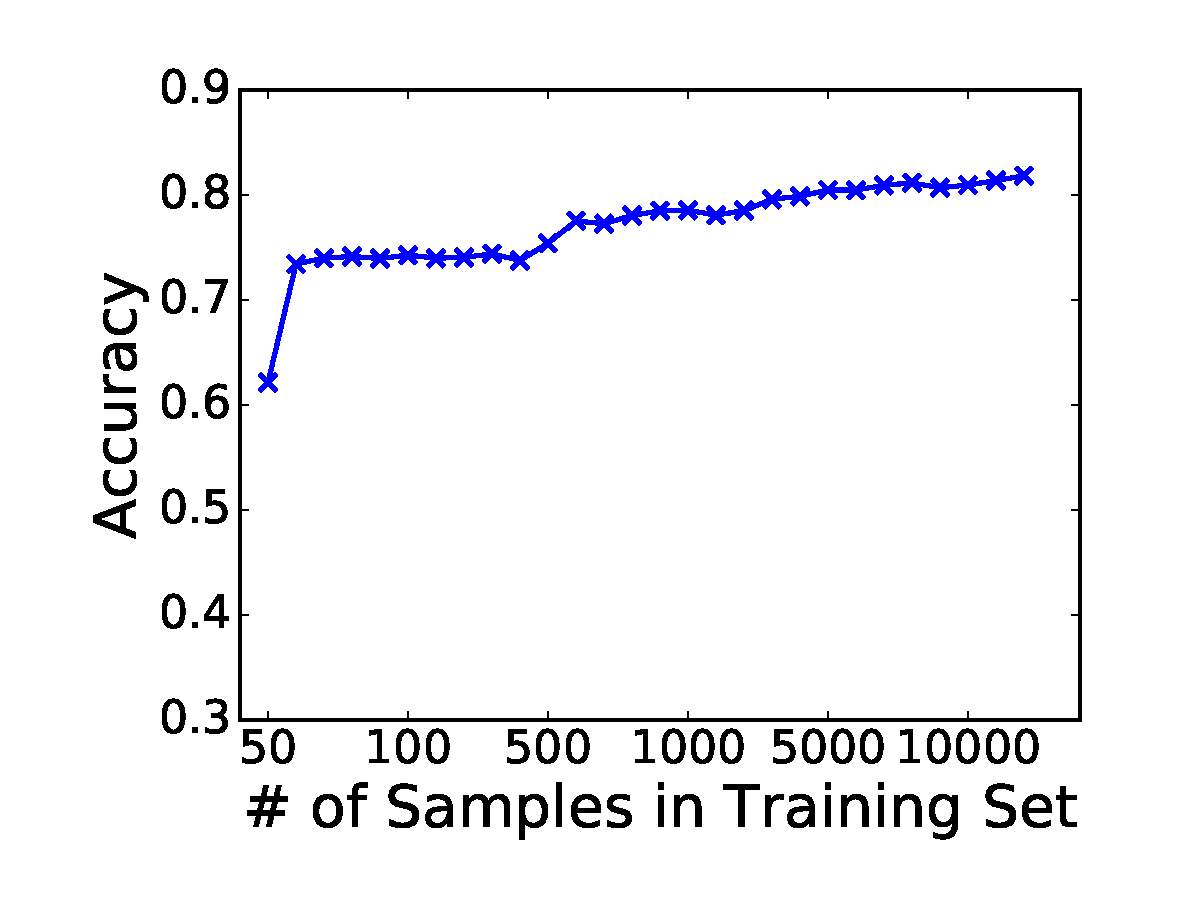
\includegraphics[width=0.16\linewidth]{figure/svm/0}\label{fig:moredata1}} 
\subfloat[Group 2]{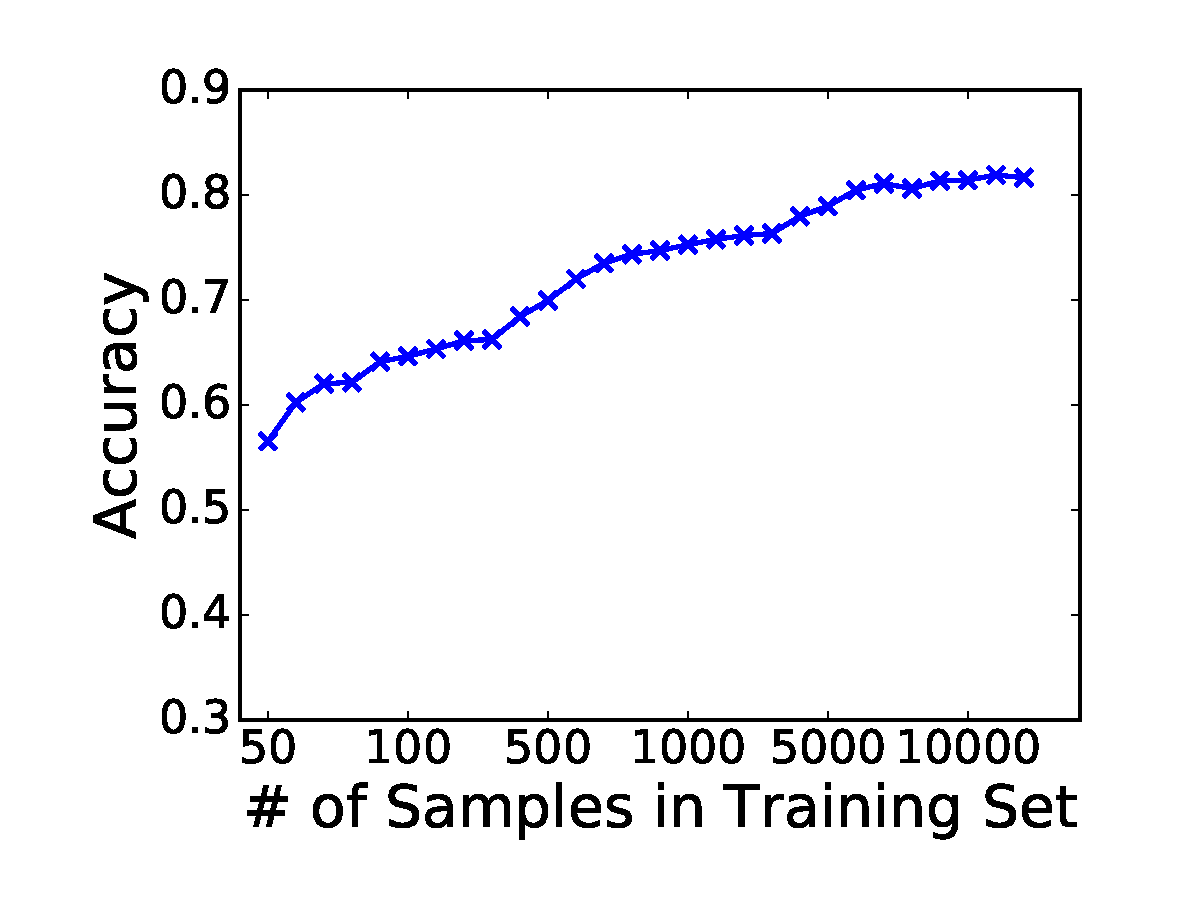
\includegraphics[width=0.16\linewidth]{figure/svm/1}\label{fig:moredata2}}
\subfloat[Group 3]{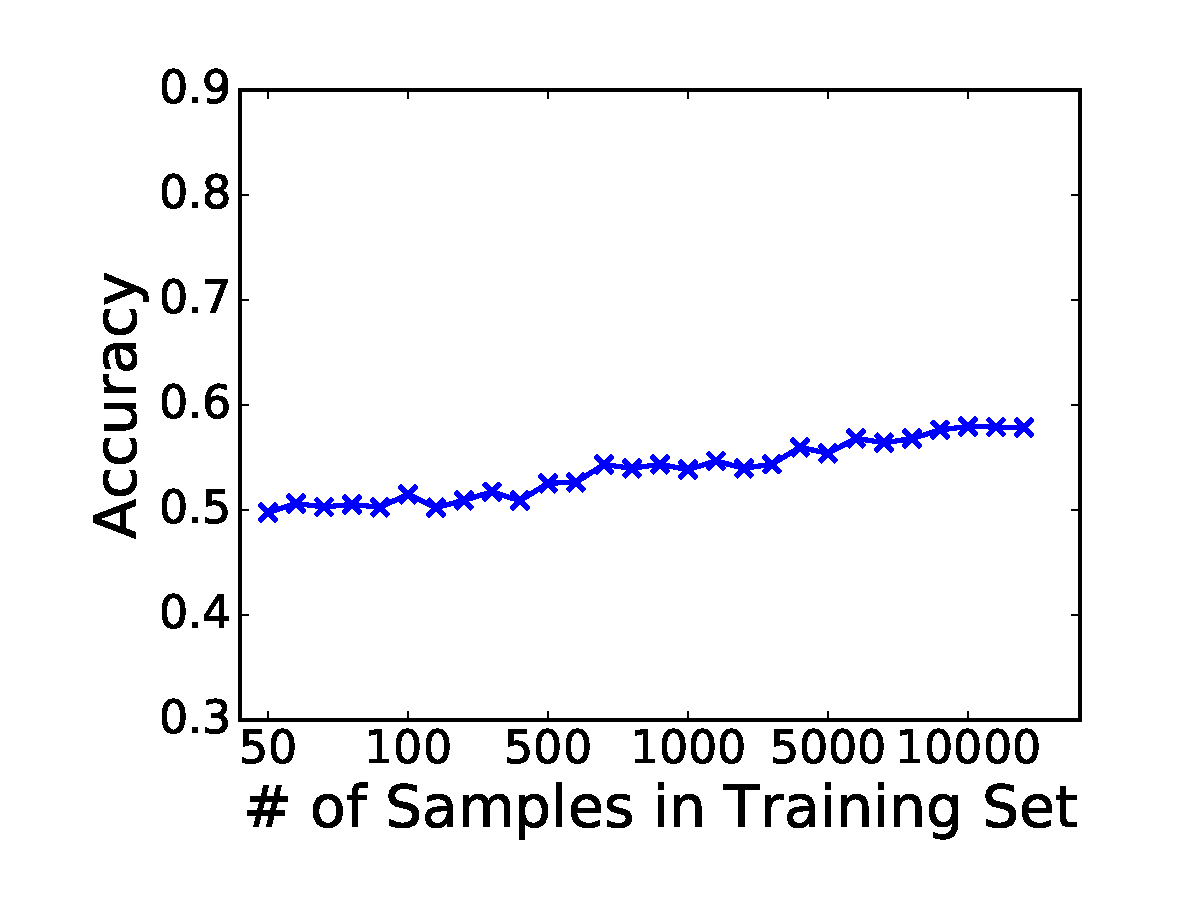
\includegraphics[width=0.16\linewidth]{figure/svm/2}\label{fig:moredata3}} 
\subfloat[Group 4]{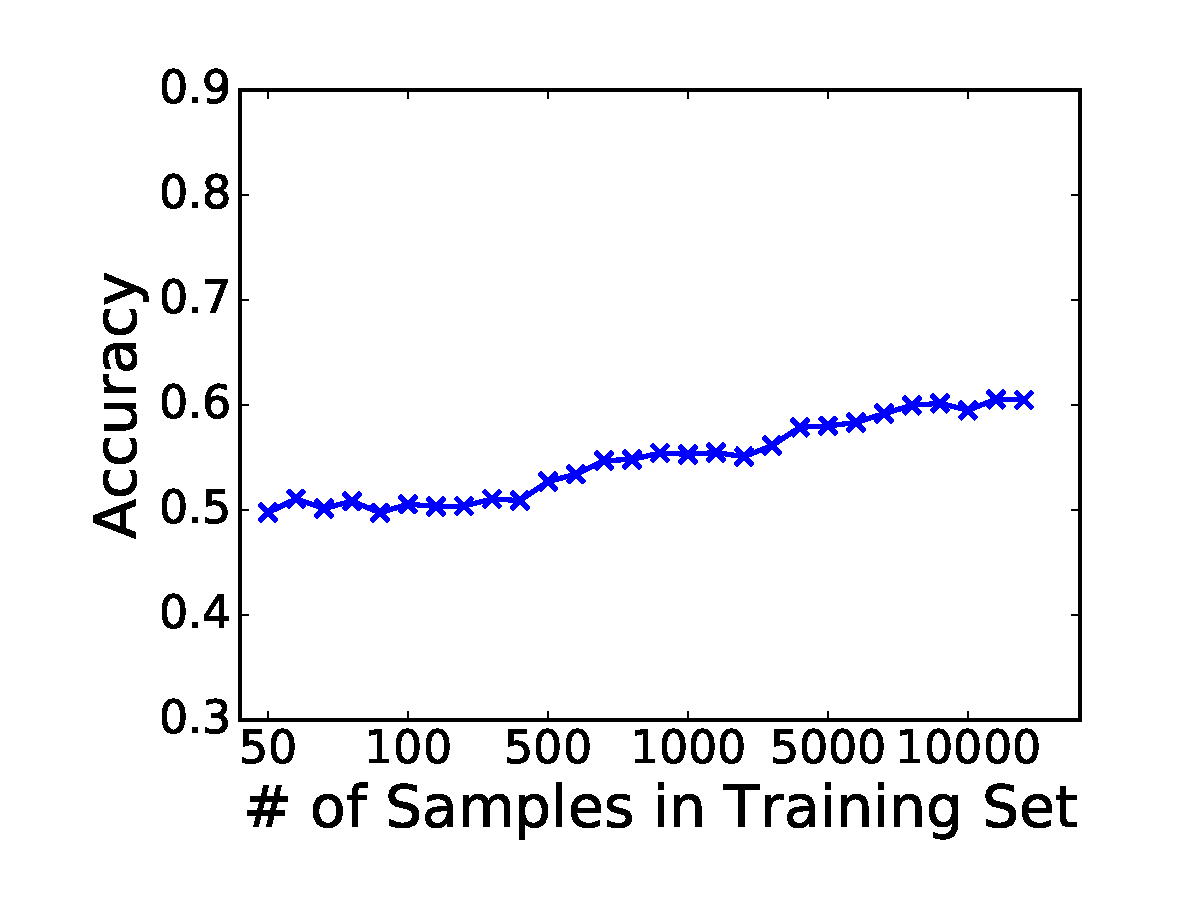
\includegraphics[width=0.16\linewidth]{figure/svm/3}\label{fig:moredata4}}
\subfloat[Group 5]{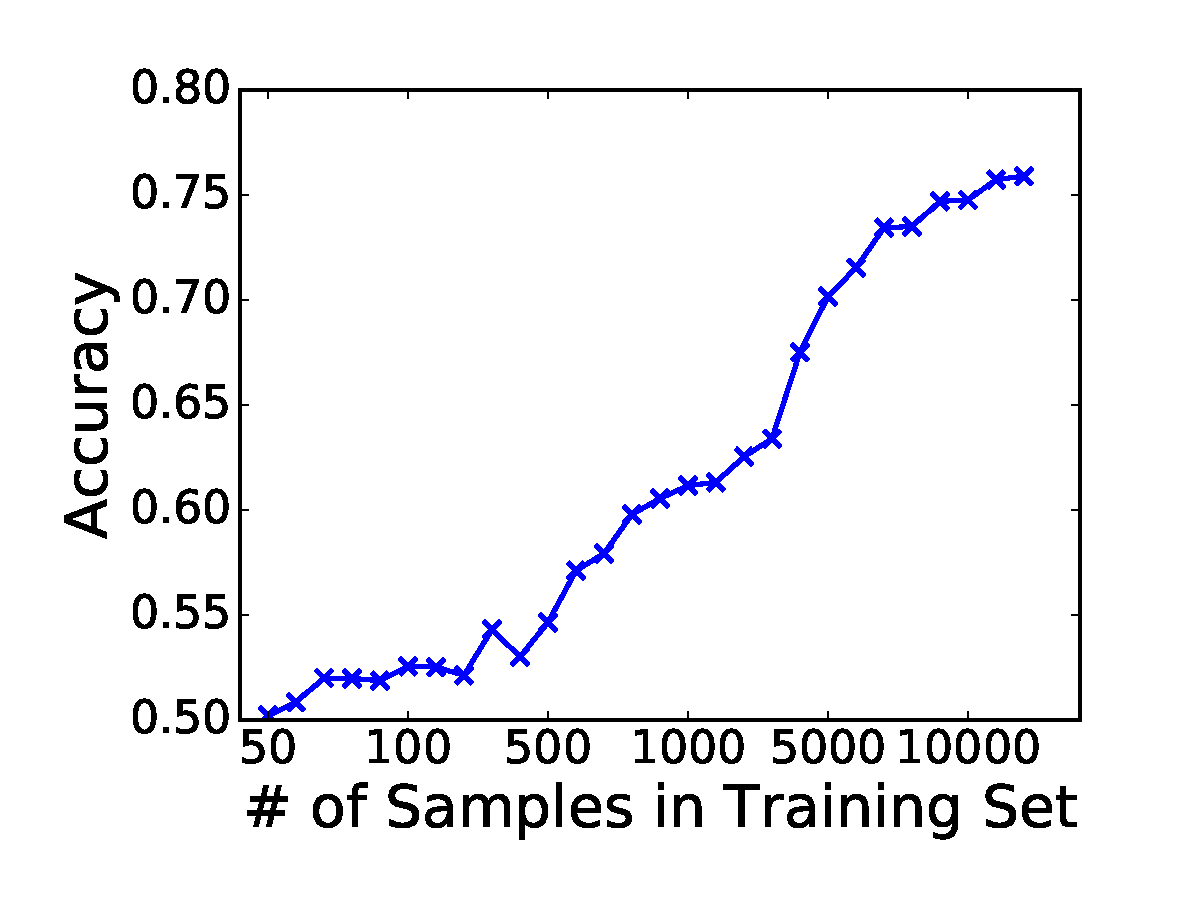
\includegraphics[width=0.16\linewidth]{figure/svm/4}\label{fig:moredata5}} \\ 

\subfloat[Group 6]{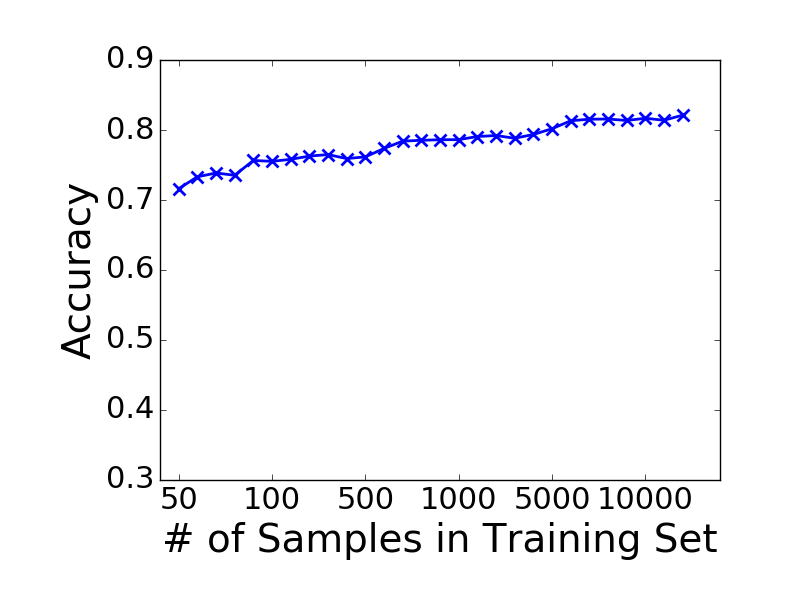
\includegraphics[width=0.16\linewidth]{figure/svm/5}\label{fig:moredata6}} 
\subfloat[Group 7]{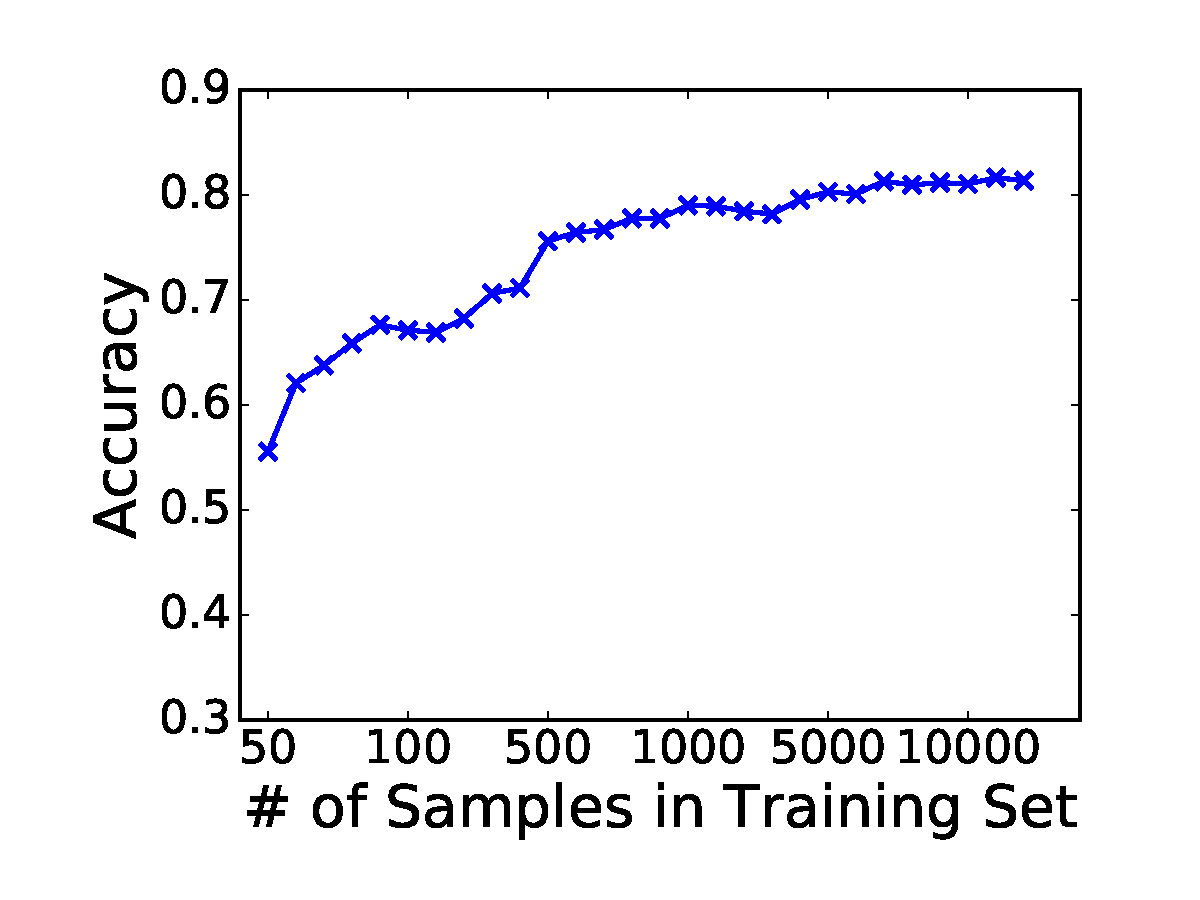
\includegraphics[width=0.16\linewidth]{figure/svm/6}\label{fig:moredata7}}
\subfloat[Group 8]{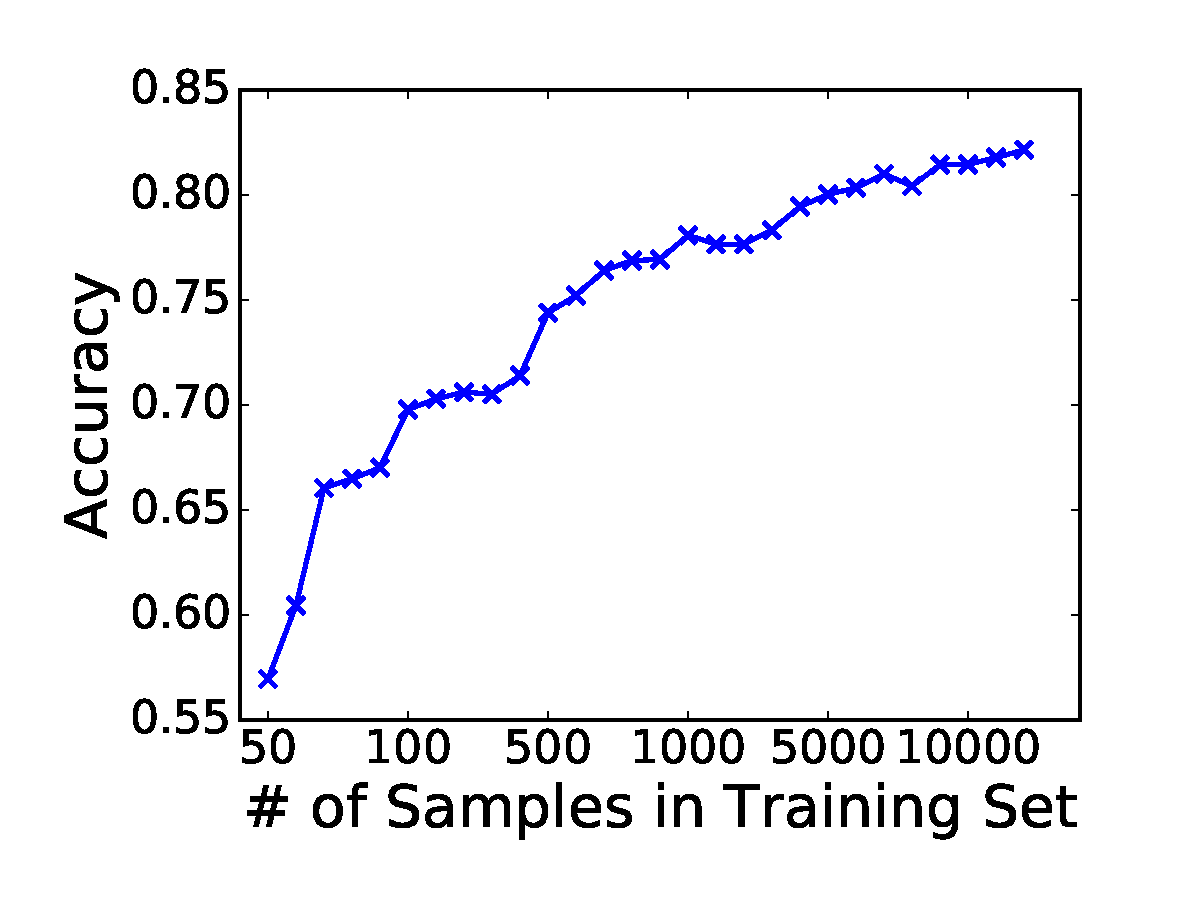
\includegraphics[width=0.16\linewidth]{figure/svm/7}\label{fig:moredata8}} 
\subfloat[Group 9]{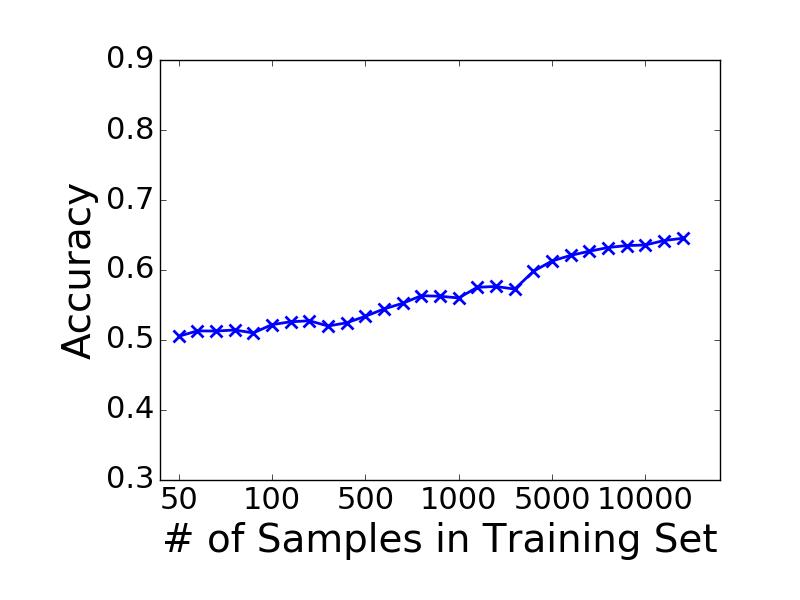
\includegraphics[width=0.16\linewidth]{figure/svm/8}\label{fig:moredata9}}
\subfloat[Group 10]{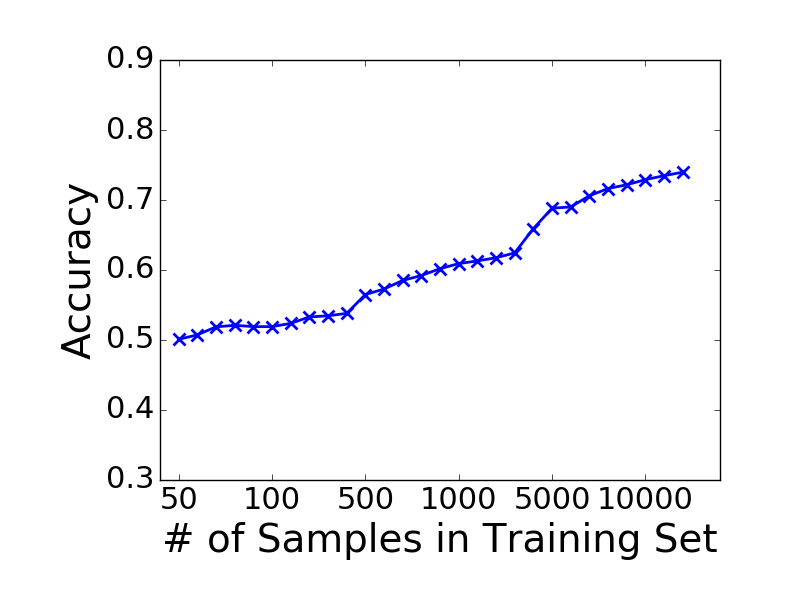
\includegraphics[width=0.16\linewidth]{figure/svm/9}\label{fig:moredata10}}
\subfloat[10-class]{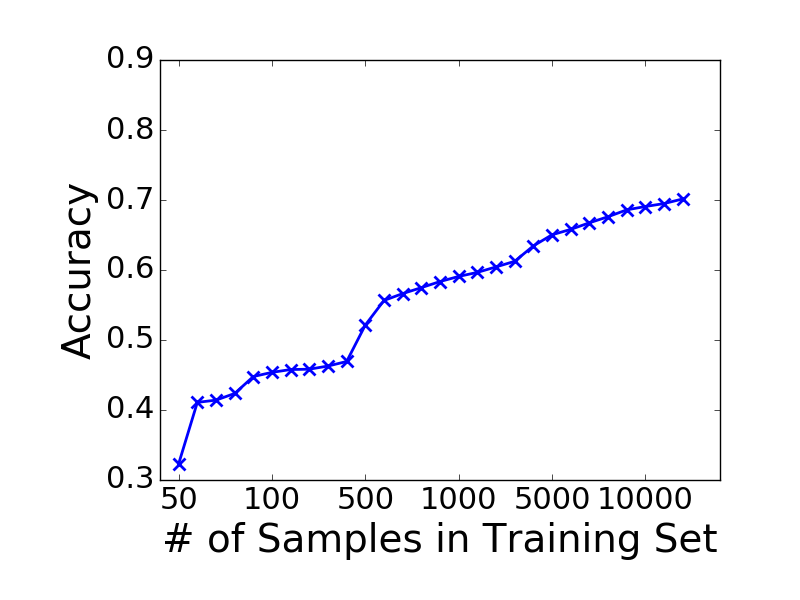
\includegraphics[width=0.16\linewidth]{figure/svm/10}\label{fig:moredata11}}
\caption{How accuracy changes with more data in traning set. 
{\footnotesize{(Figure~\ref{fig:moredata1} - Figure~\ref{fig:moredata10} show how accuracy of each two-class classifier changes 
with the size of training set changing from 50 to 10000. 
Figure~\ref{fig:moredata11} shows how accuracy of the ten-class classifier changes with the size of training set increaing from 50 to 10000. )}}} 
\label{fig:moredata} 
\end{figure*} 

%\subsection{Classification Experiments}


\subsection{Discussion}
1. Future work about indexing ssdeep string
2. Upper bound
3. More data better results
4. Need human effort or dynamic information 
\section{Related Works}
\label{sec:related}

\subsection{Leveraging Source Code Repositories}

Recently, there have been many works on exploring how to leverage open-source code repositories that contain vast amount of source code projects, 
such as GitHub, BitBucket, and CodePlex. 
SLANG~\cite{code-completion} trains statistical models using extracted sequences of API calls from large code bases
and applies the trained models to fill uncompleted programs with call innovations. 
JSNICE~\cite{big-predicting} aims to predict identifier types and obfuscated identifier names for JavaScript programs. 
A score function based on learned CRF model is optimized to make all predictions. 
Phrase-based statistical translation approaches have also been proposed
to translate C\# programs to Java programs~\cite{big-translation}. 

These systems analyze source codes by leveraging large code bases in open-source code repositories.
We have different objectives and methods: 
we analyze malwares and anti-virus engines by leveraging an open malware repository.
%and we rely on malwares’ metadata information and ssdeep hash strings calculated from binary executables.


\subsection{Analyzing and Leveraging VirusTotal}
We are not the first to investigate \vt.
The research community starts to pay more attention to VirusTotal repository recently
and there have been several works on \vt.

The closest relaed work is a recent study on \vt{}~\cite{SongAPsys2016}. 
Similar to our work, they downloaded one-month data from VirusTotal
and focused on PE files.
They studied a set of basic properties of PE malwares,
including size distribution, malware family distribution, and temporal properties.   
We collected a longer period of data from \vt.
More important, we performed deeper analysis into what are the fundamental factors 
that correlate and influence malware detection.
Apart from studying malwares, we also study anti-virus engines and how they influence each other
and perform classification and clustering on \vt\ data.
These findings provide far more insights than the previous work and will be able to help future researchers more.
%Different from our work, 
Finally, the previous work only relied on detection results from Microsoft anti-virus engines,
while we conducted our study using all engines.
%study correlations between metadata and detection results from all engines, 
%and we also evaluate different detection engines by modeling influence among different engines.  

Recently, researchers noticed that some malware writers use VirusTotal as testing platform~\cite{huangvt2016bigdata, neeles}.
They explored this phenomenon and developed techniques to identify malware writers. 
Huang \etal\ downloaded four months of VirusTotal metadata to identify Android malware development cases~\cite{huangvt2016bigdata}. 
Their technique first alerts suspicious source IDs 
and then conducts program analysis to further validate whether 
these source IDs are really testing their Android malware prototypes on \vt{}. 
Graziano \etal\ tried to identify Windows malware development cases on Anubis~\cite{neeles}. 
They used data on VirusTotal to validate their findings. 
{\color{red} Their works target to identify suspicious source IDs, 
while we focus on understanding correlations between source IDs' history and detection rate of their submissions.} 
%Their works focus on submission history of each source ID, 
%while we \yiying{fill}.  

Kantchelian \etal\ applied various supervised and unsupervised 
techniques to aggregate various labels from different anti-virus engines into one ground truth label 
on a dataset collected from VirusTotal~\cite{betterGT}. 
Their goal is to find better ground truth label for distinct samples, 
while our work tries to model influence among different anti-virus vendors.  

%3. Code classification and clustering





%\input{related}
%\input{conclusion}

%%\balance
%\begin{spacing}{0.65}

\balance
{
\bibliographystyle{abbrvnat}
\bibliography{security} 
}
%\end{spacing}
\end{document}

% Local variables:
% TeX-PDF-mode: t
% TeX-master: t
% End:

% LocalWords:  Crug cci
